\documentclass[12pt]{beamer}

    \usepackage[utf8]{inputenc}
    \usepackage{graphics}
    \usepackage{listings}
    
    \usepackage{array,booktabs}
    
    \usetheme{Madrid}
    \usecolortheme{beaver}
    
    % custom commands
    \newcommand{\nologo}{\setbeamertemplate{logo}{}} % set logo to empty
    
    \title{New Zealand Trip}
    \author{Arun}
    \date{\today}
    
    
    \logo{\includegraphics[height=1.0cm]{images/logo.png}}
    
    \begin{document}
        \frame{\titlepage}
        \begin{frame}
            \begin{center}
                \includegraphics[width=1\textwidth]{images/road-trip.png}
            \end{center}
        \end{frame}
    
        \begin{frame}
            \frametitle{My Trip}
            %\begin{columns}
                %\column{0.5\textwidth}
                \begin{center}
                    \includegraphics[height=0.6\textheight]{images/camper-van.jpg}<1>
                    \includegraphics[height=0.6\textheight]{images/map.png}<2>
                    \includegraphics[height=0.6\textheight]{images/mt-cook-road.jpg}<3>
                \end{center}
    
                %\column{0.5\textwidth}
                \begin{itemize}
                    \item In a Camper van for 17 days
                    \pause
                    \item This was the road trip (13 places)
                    \pause
                    \item And the road
                \end{itemize}
            %\end{columns}
        \end{frame}

        \begin{frame}
            \frametitle{Weather}
            %\begin{columns}
                %\column{0.5\textwidth}
                \begin{center}
                    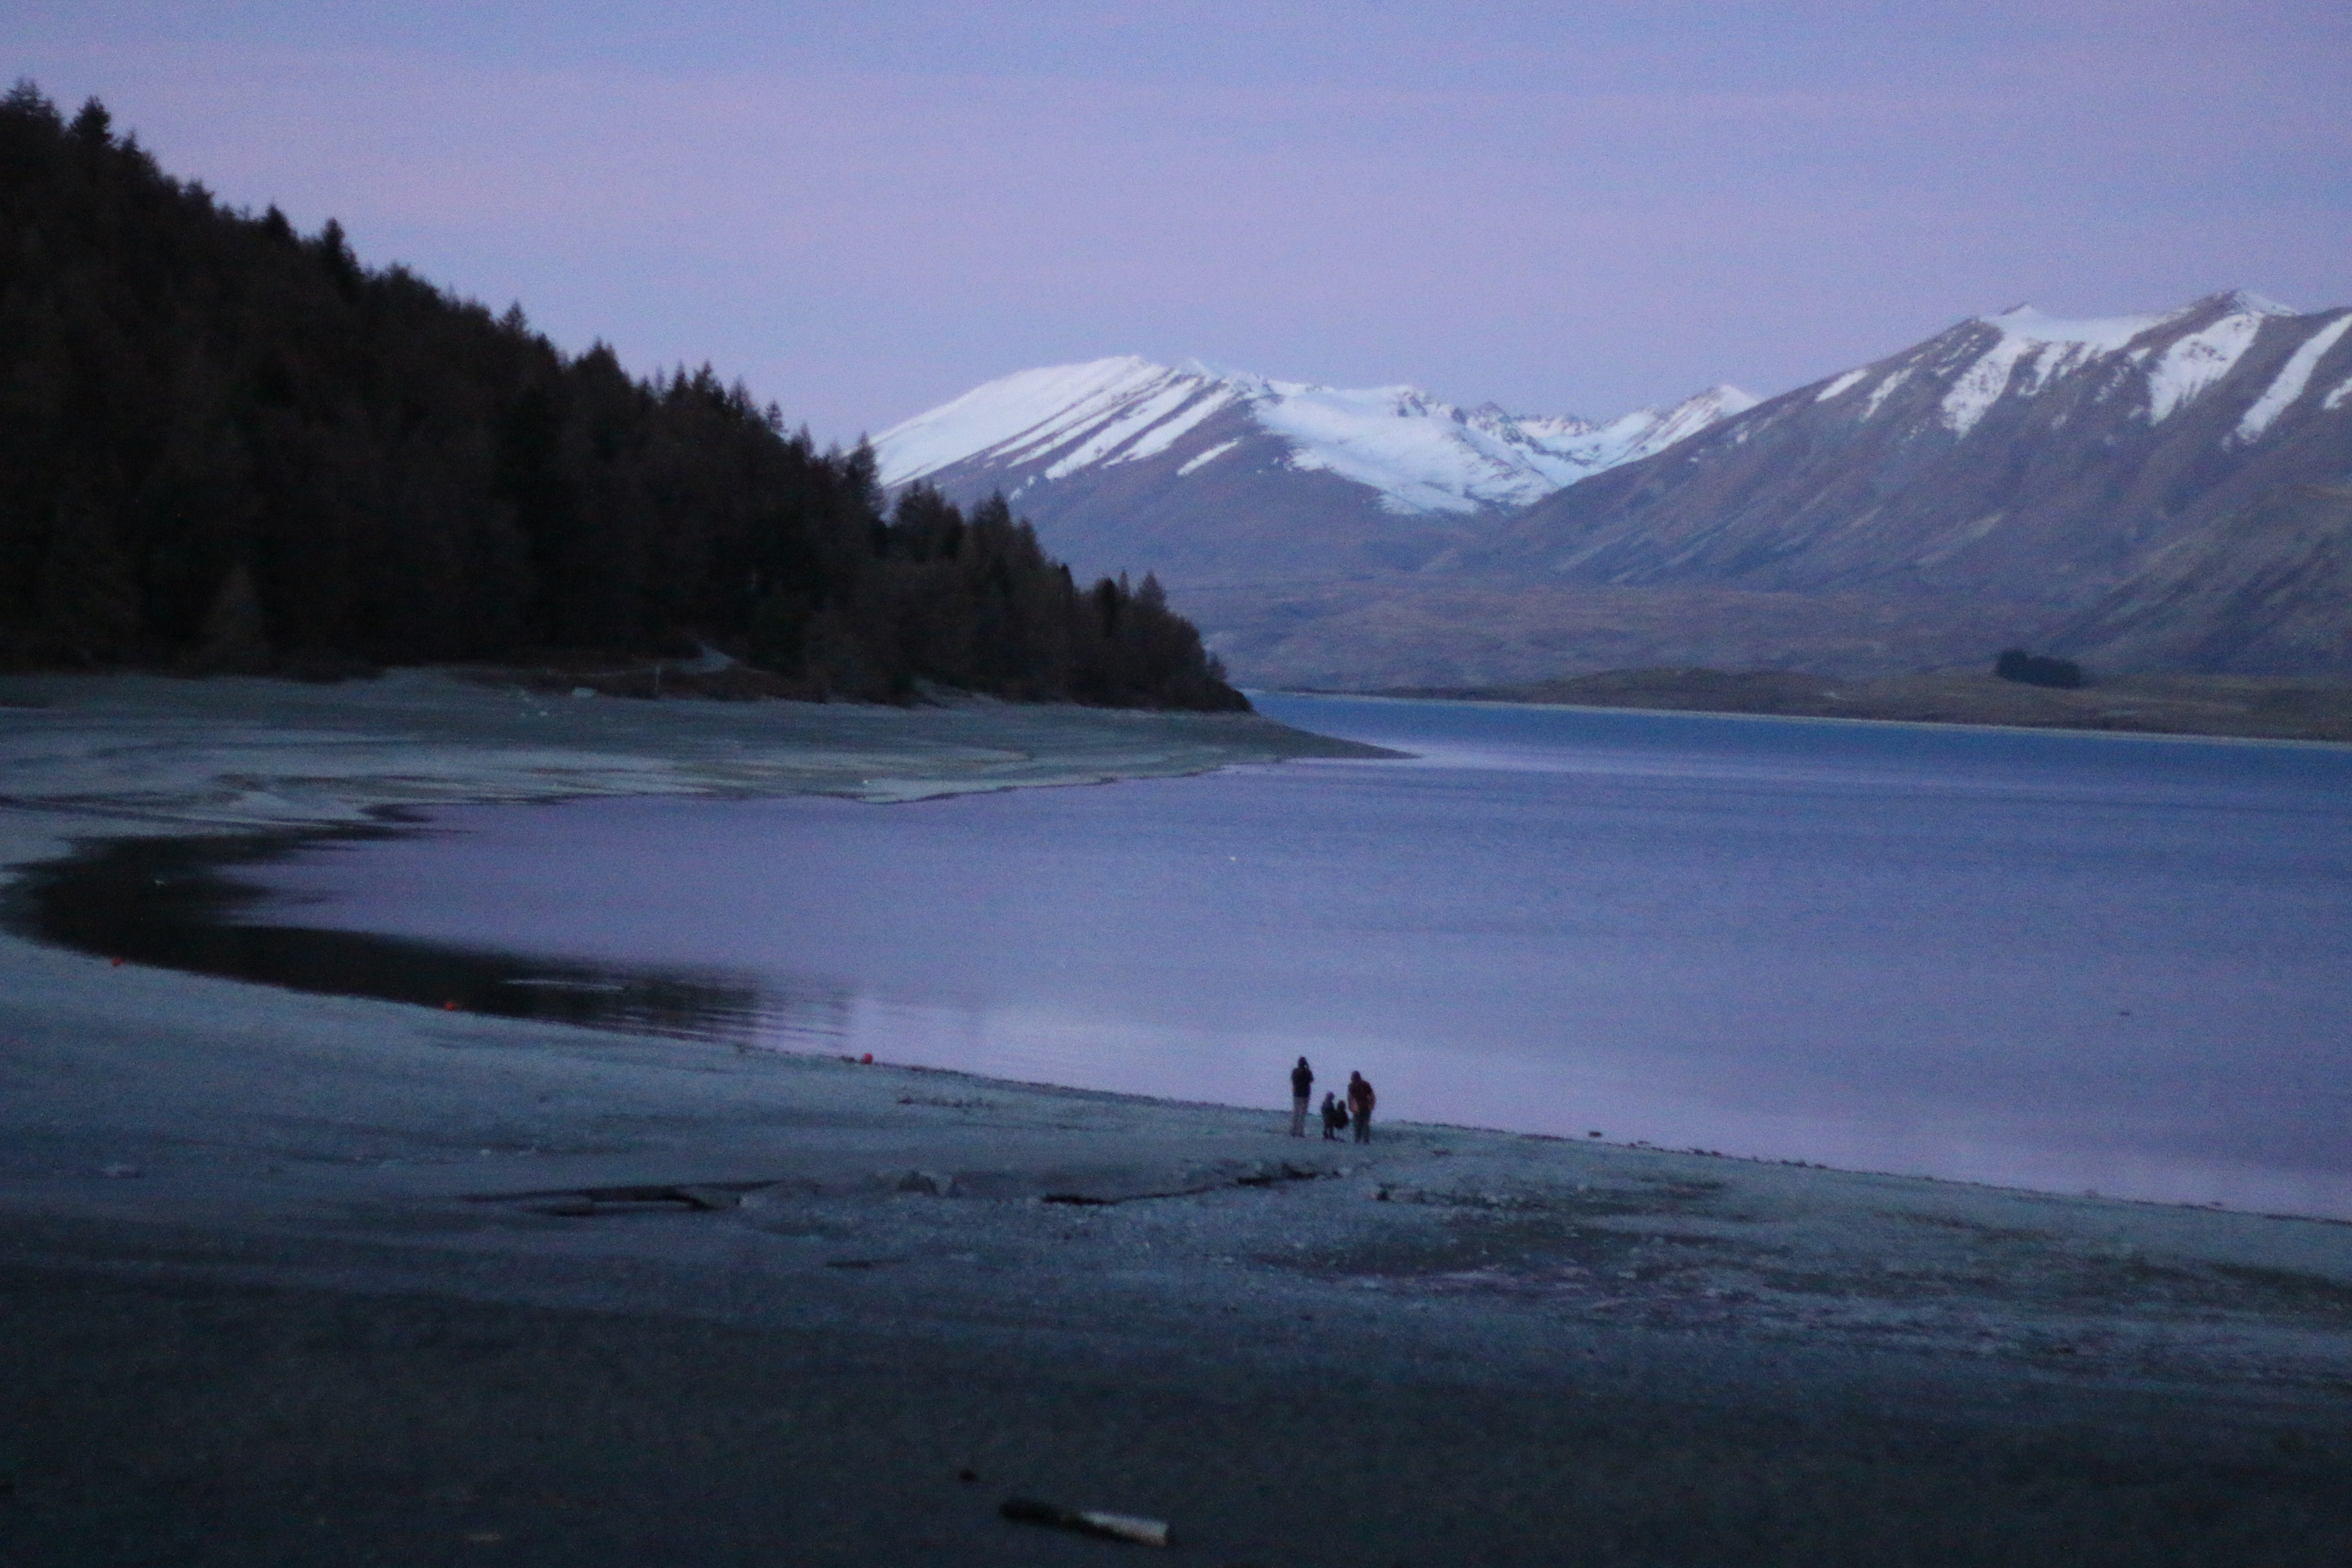
\includegraphics[height=0.6\textheight]{images/teakapo-2.JPG}<2>
                    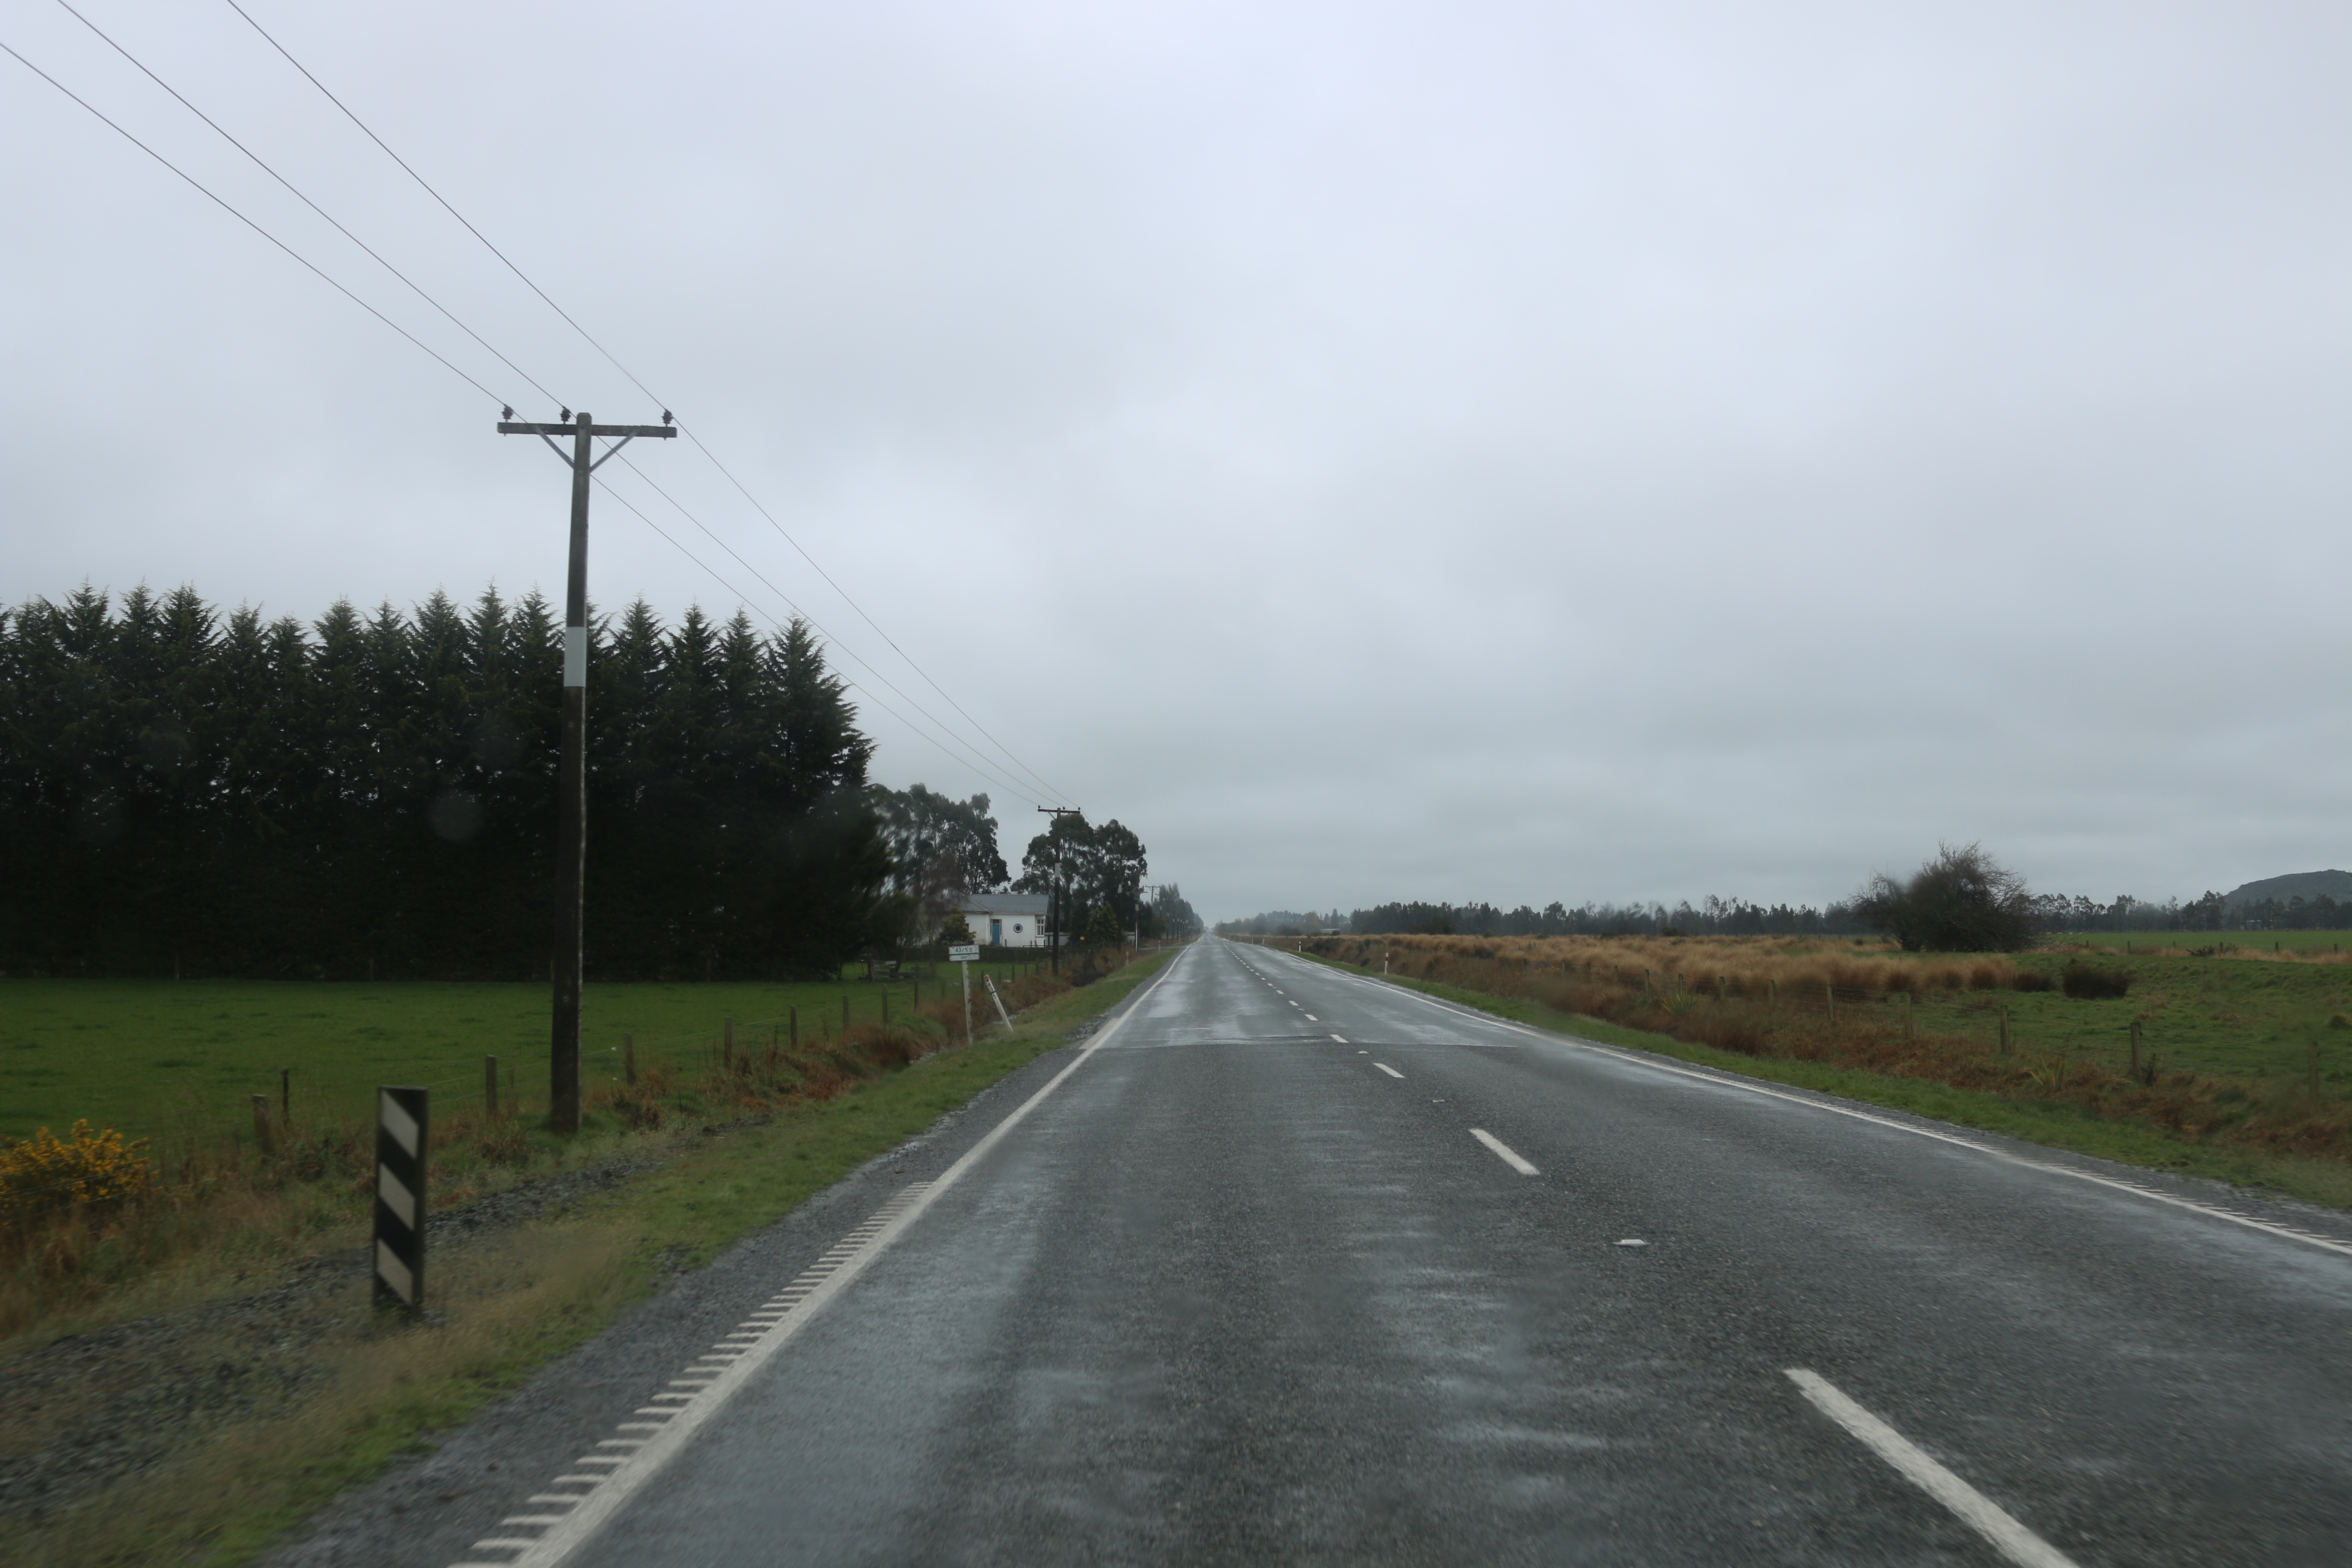
\includegraphics[height=0.6\textheight]{images/road-rain.JPG}<3>
                    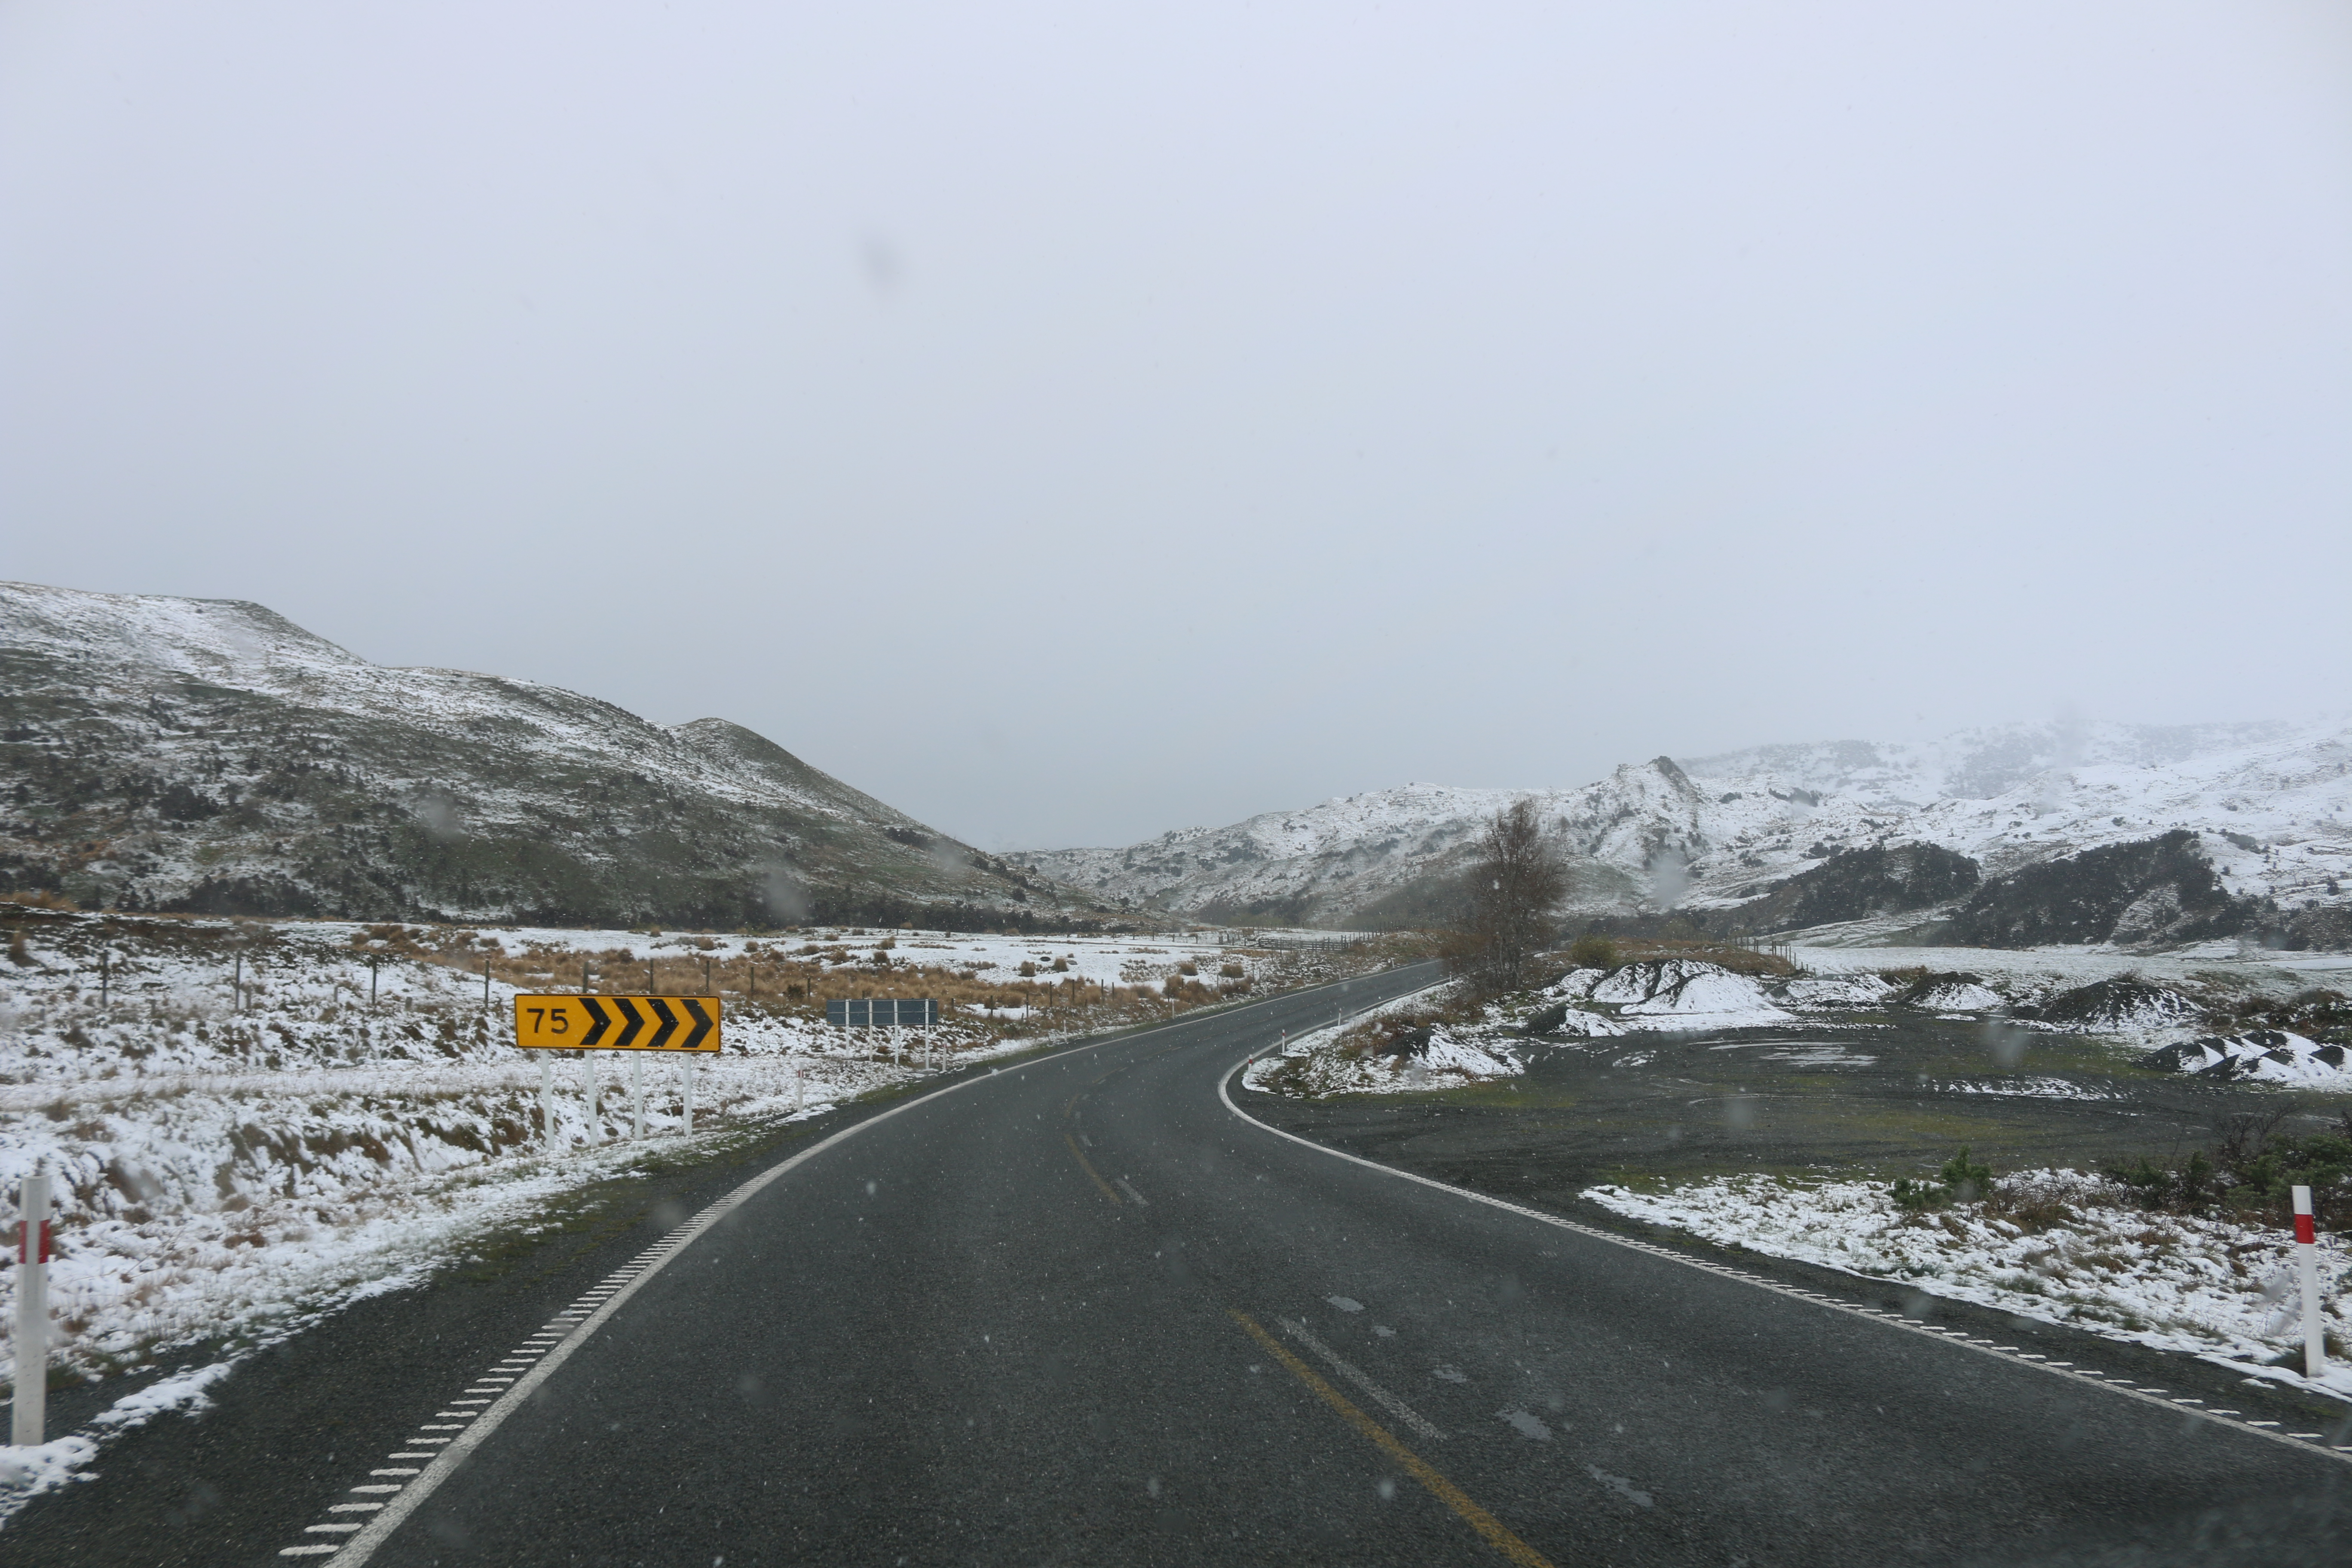
\includegraphics[height=0.6\textheight]{images/road-snow.JPG}<4>
                \end{center}
            
                %\column{0.6\textwidth}
                \begin{itemize}
                    \item Started warm and sunny
                    \pause
                    \item 2$^\circ$ C and windy
                    \pause
                    \item rainy
                    \pause
                    \item and it snowed as well (all in first 3 days)
                \end{itemize}
            %\end{columns}
        \end{frame}

        \begin{frame}
            \frametitle{Best Campsite}
            %\begin{columns}
                %\column{0.5\textwidth}
                \begin{center}
                    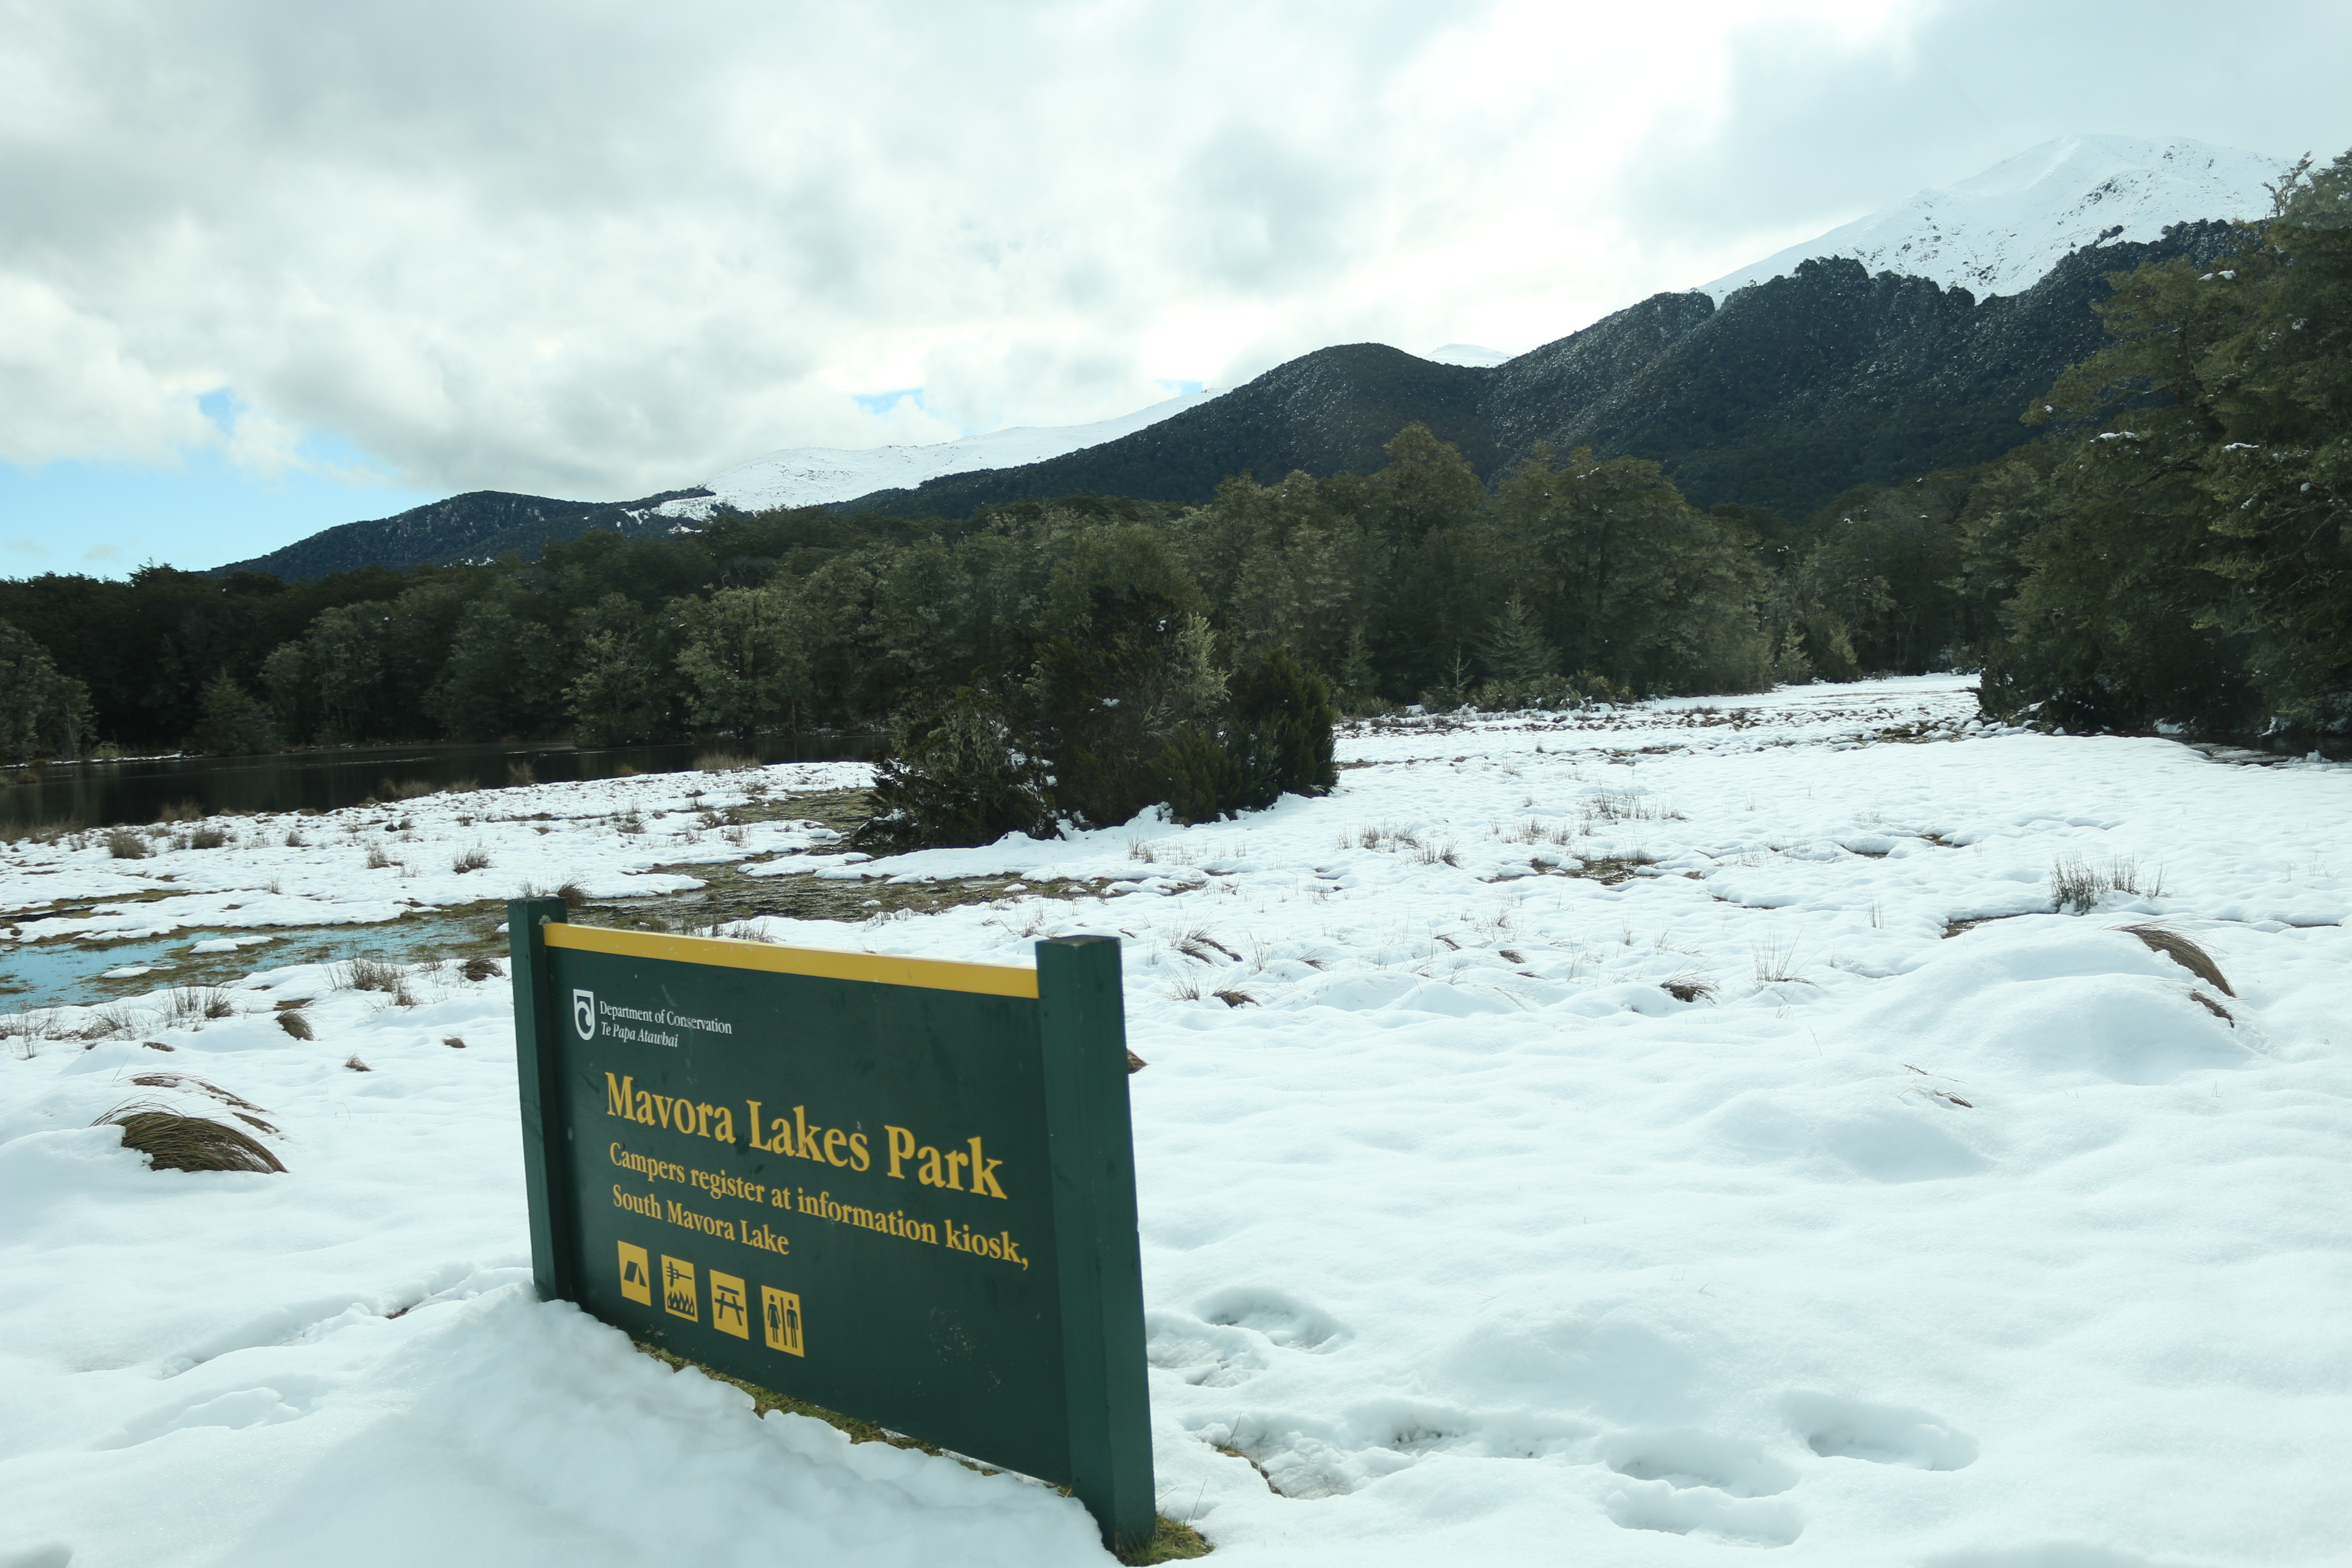
\includegraphics[height=0.6\textheight]{images/mavora-camp.JPG}<1>
                    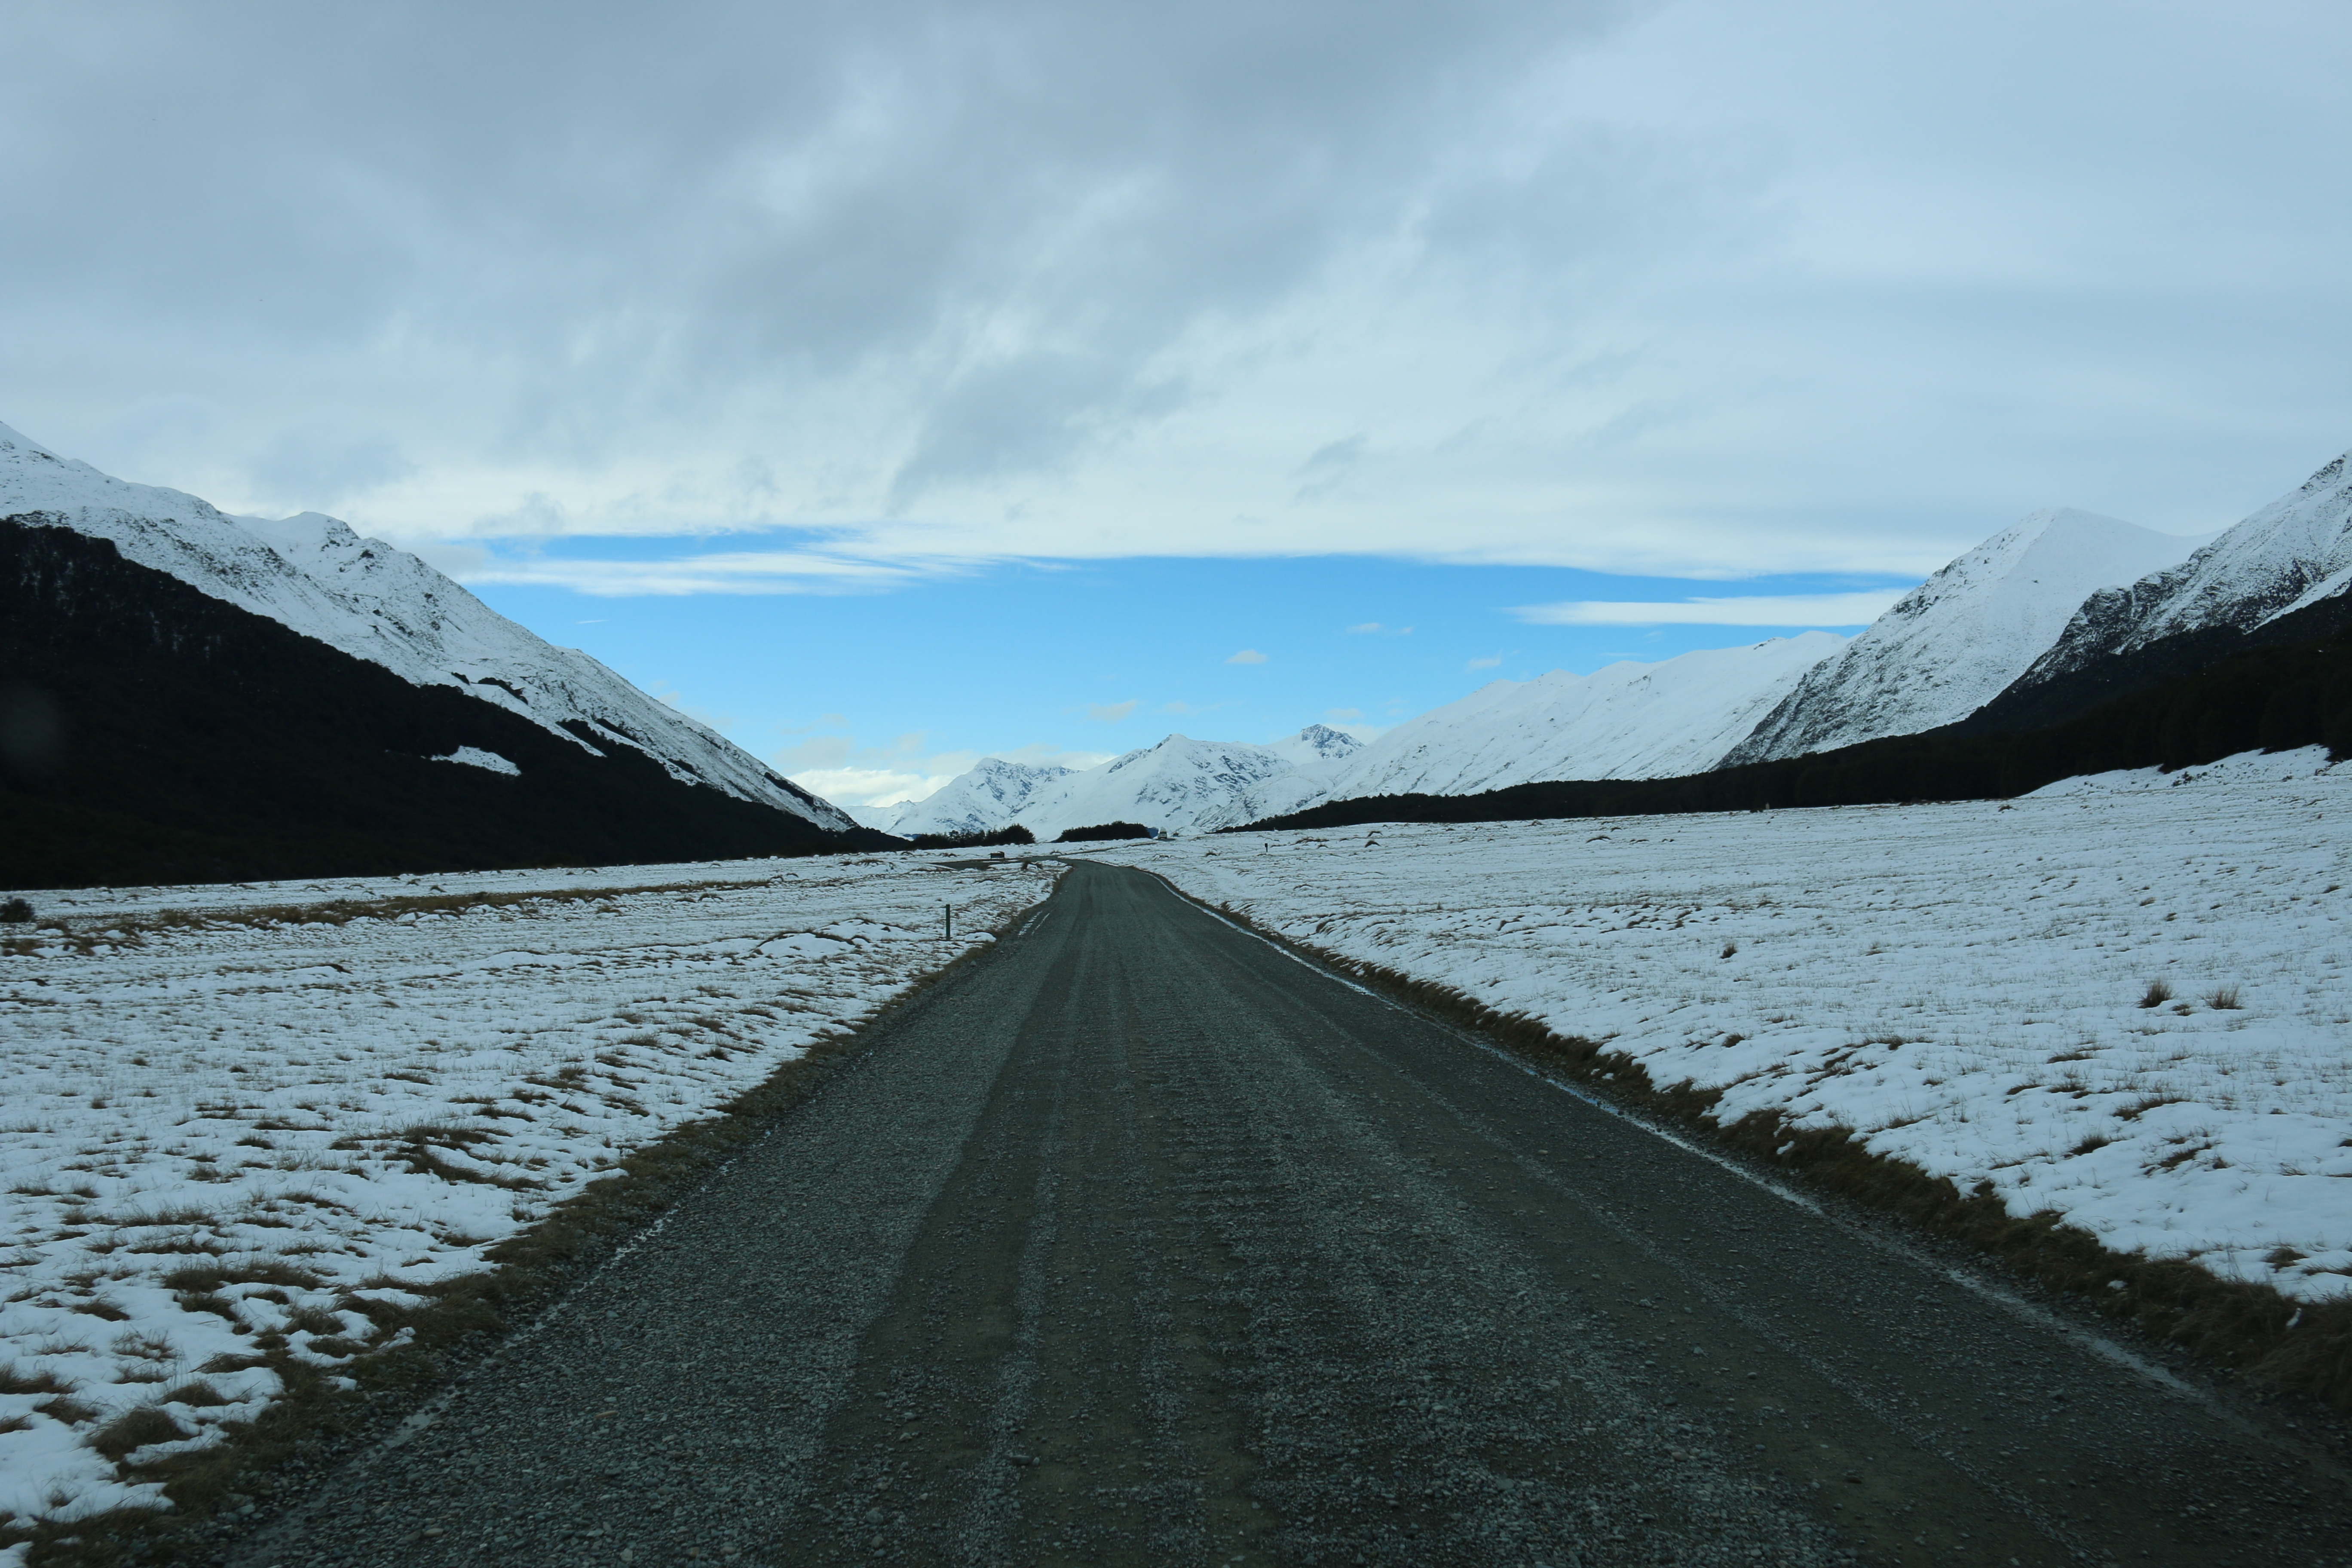
\includegraphics[height=0.6\textheight]{images/to-mavora.JPG}<2>
                    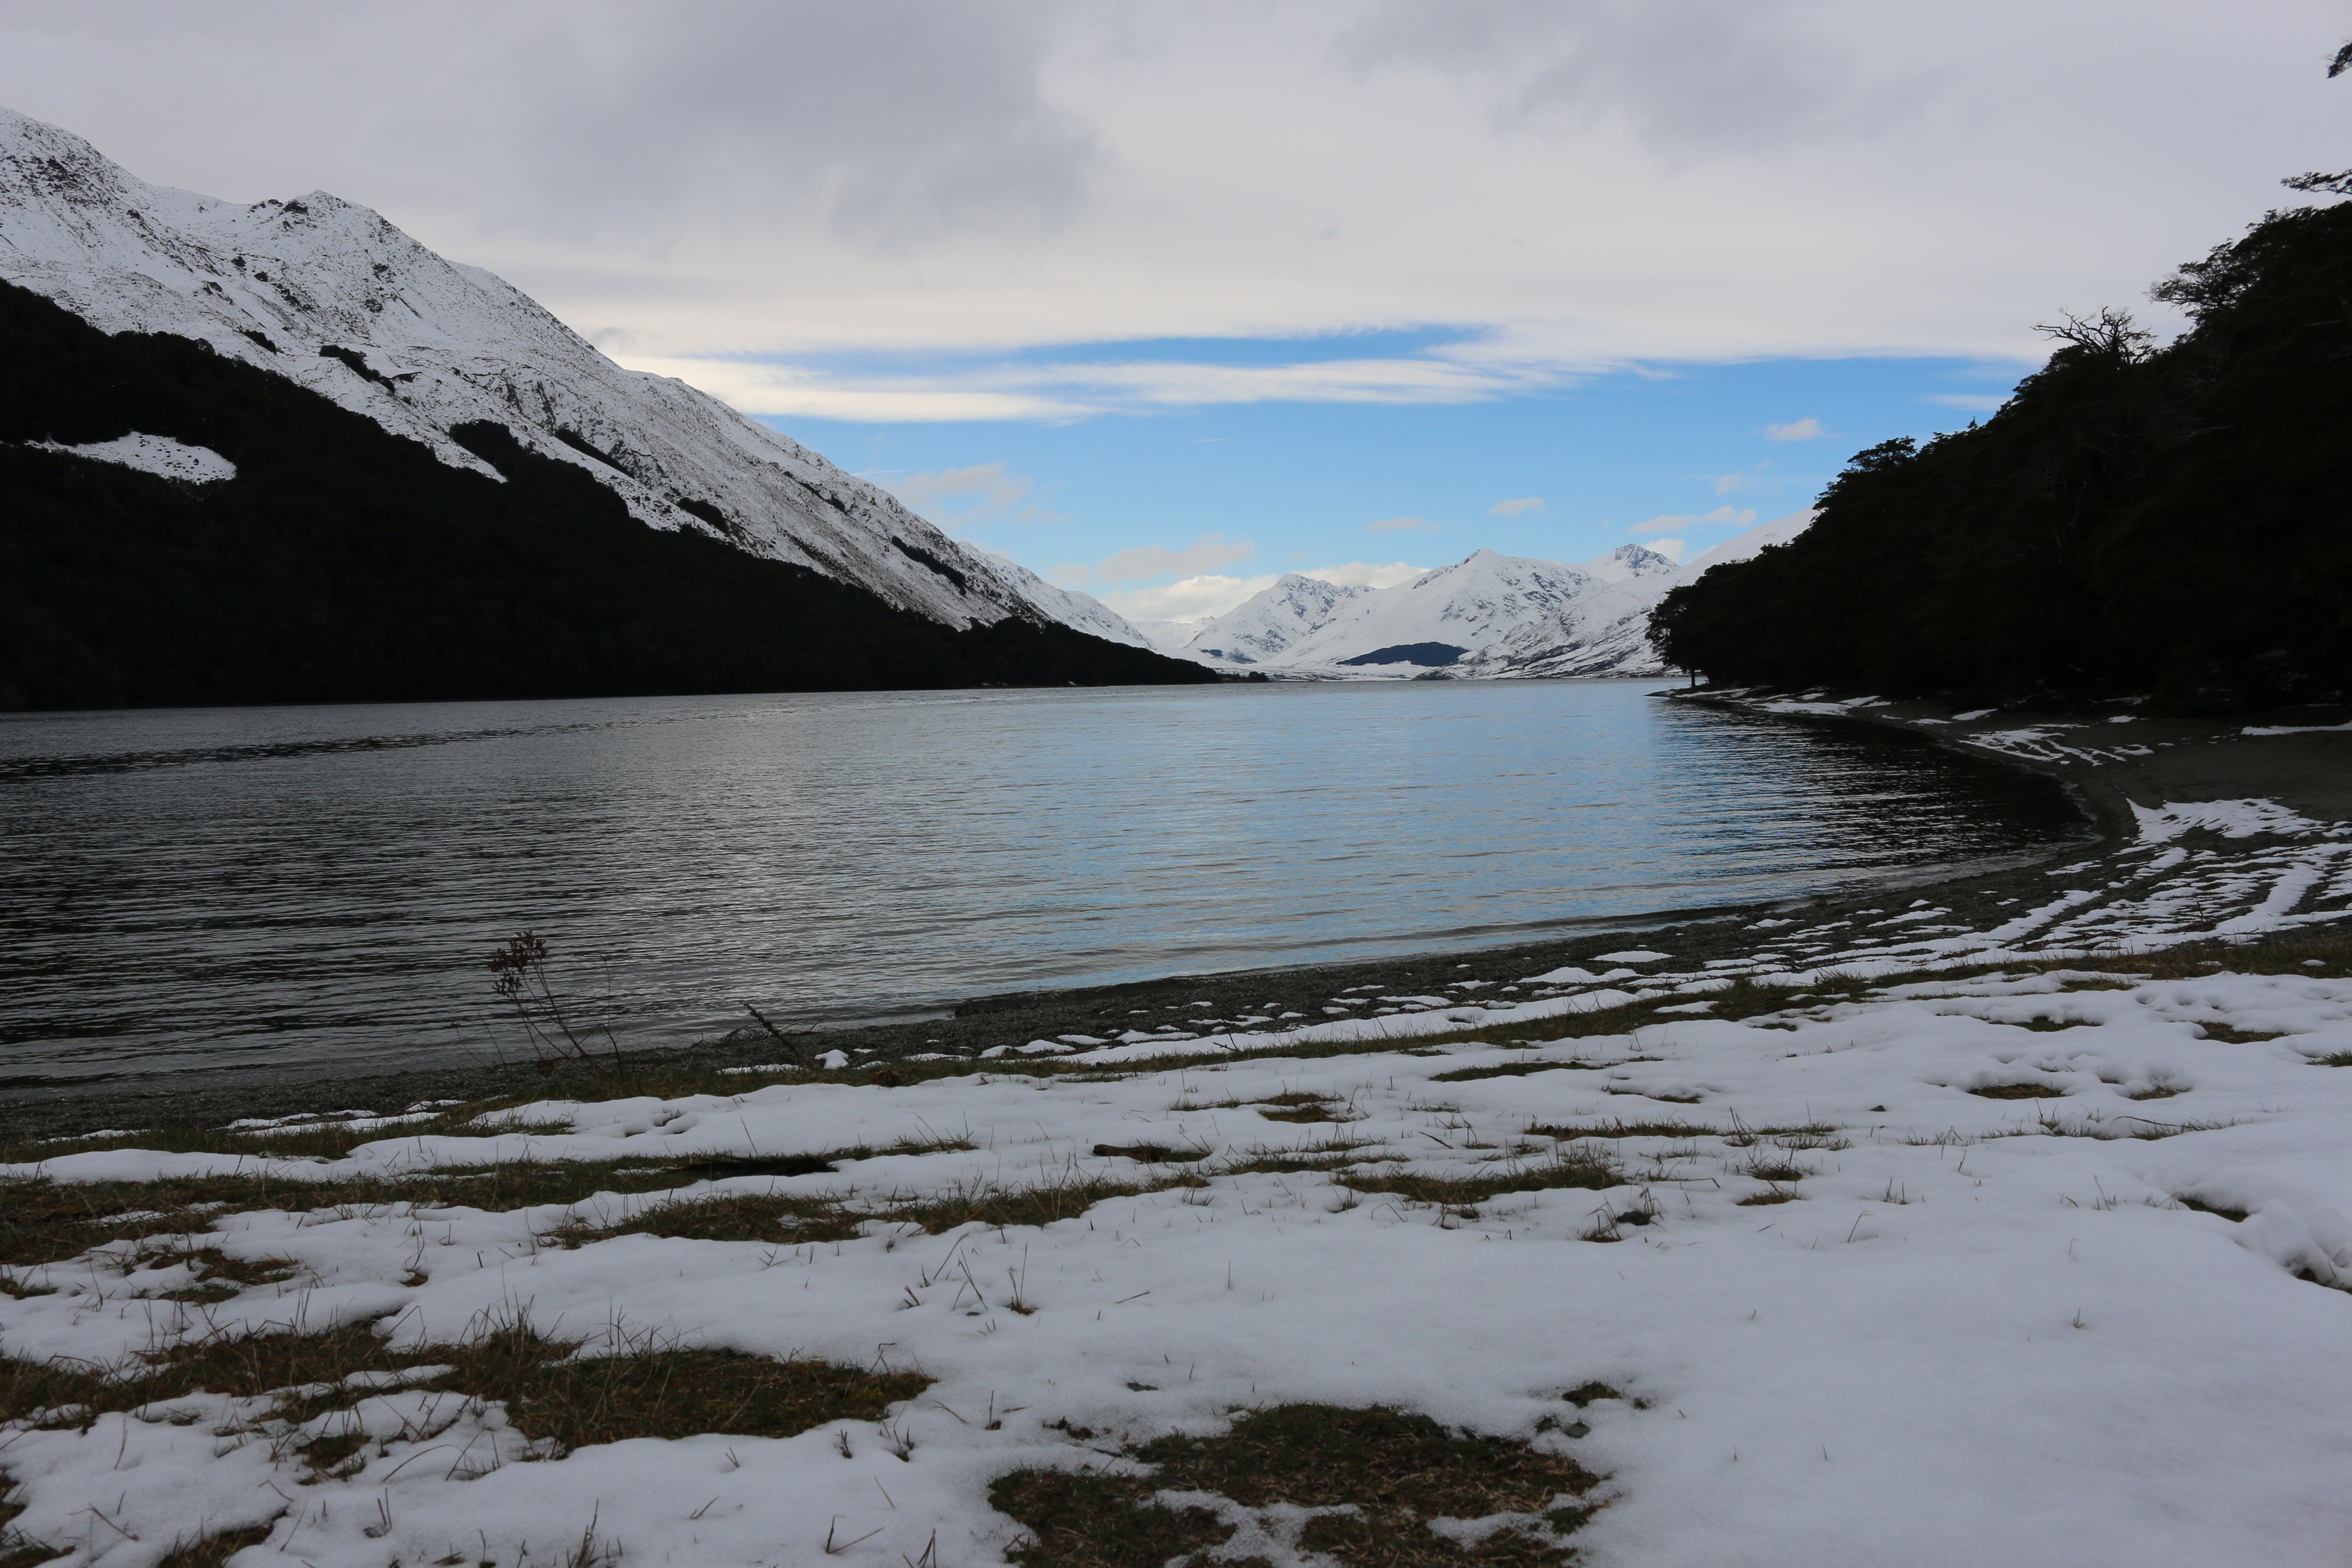
\includegraphics[height=0.6\textheight]{images/mavora-lake.JPG}<3>
                    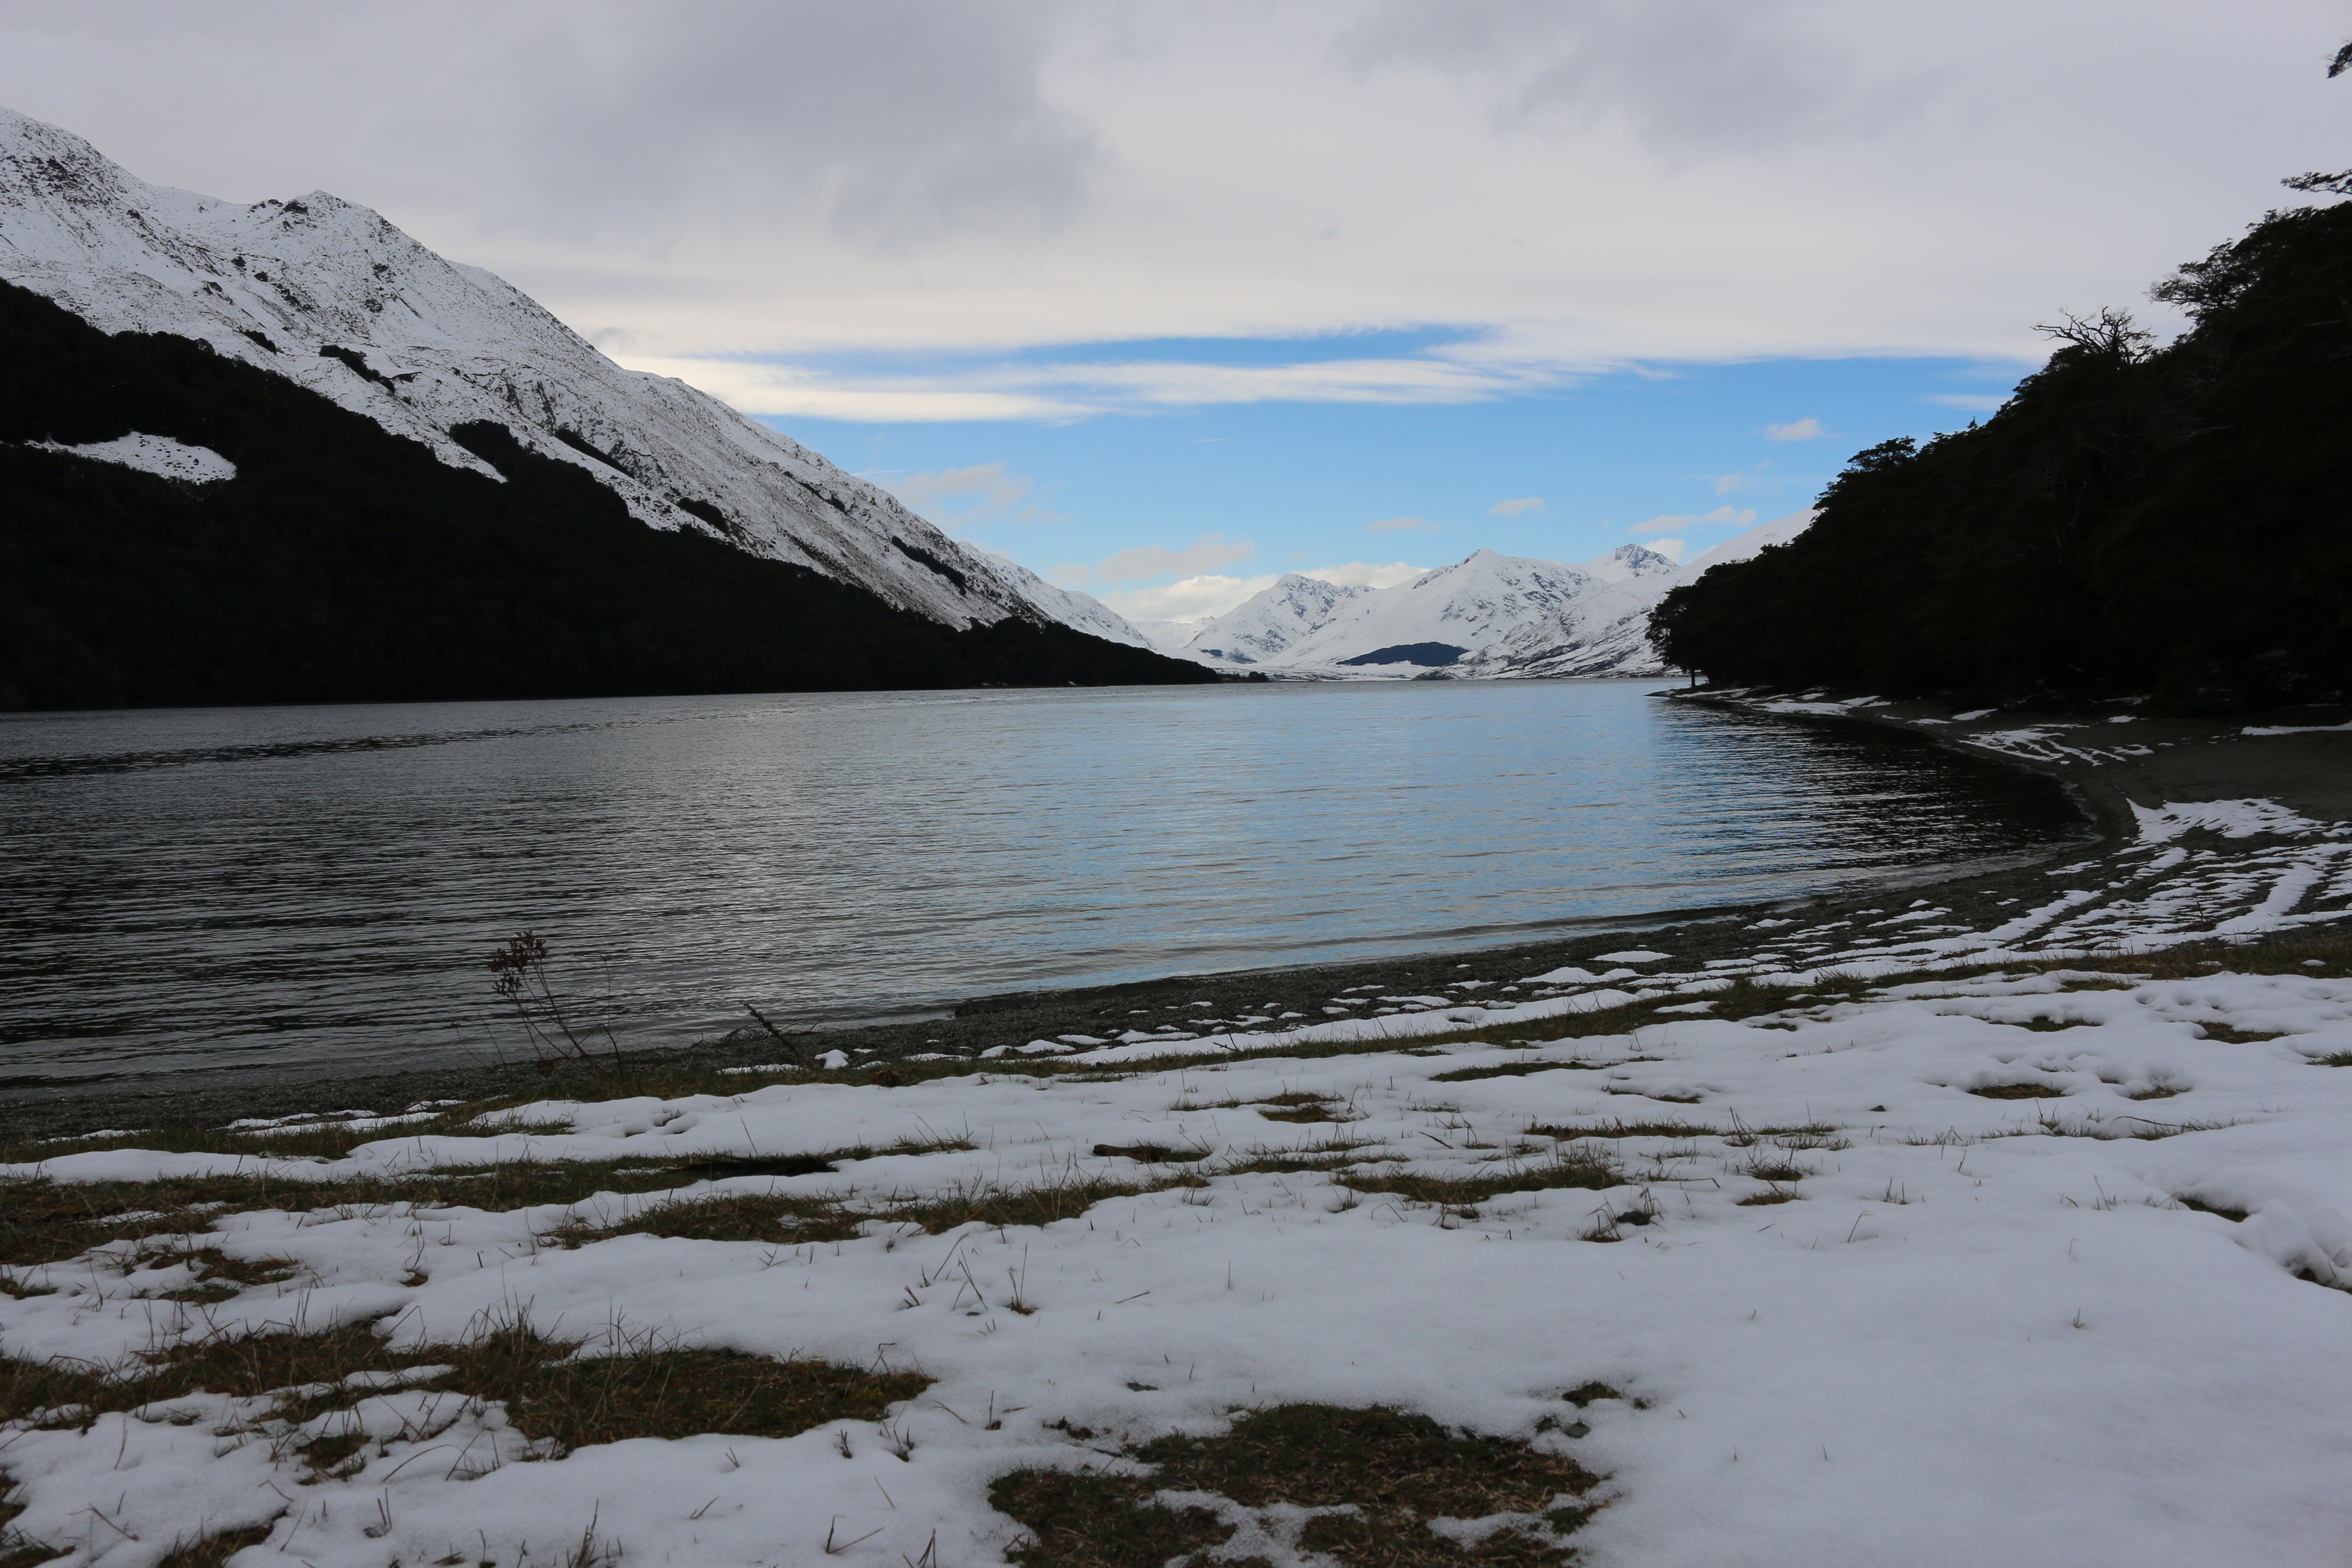
\includegraphics[height=0.5\textheight]{images/mavora-lake.JPG}<4>
                \end{center}
            
                %\column{0.6\textwidth}
                \begin{itemize}
                    \item Mavora Lakes
                    \pause
                    \item 50 kms of gravel single lane road
                    \pause
                    \item That's the view from where I was camping
                    \pause
                    \item This is the spot where Frodo and Sam break away from the Fellowship by crossing to the eastern shore on an elven boat.
                \end{itemize}
            %\end{columns}
        \end{frame}

        \begin{frame}
            \frametitle{Milford Sounds}
            %\begin{columns}
                %\column{0.5\textwidth}
                \begin{center}
                    \includegraphics[height=0.5\textheight]{images/milford-sounds.jpg}<1>
                    \includegraphics[height=0.5\textheight]{images/homer-tunnel.jpg}<2>
                    \includegraphics[height=0.5\textheight]{images/milford-sounds-map.jpg}<3>
                    \includegraphics[height=0.5\textheight]{images/milford-sounds.jpg}<4>
                \end{center}
            
                %\column{0.6\textwidth}
                \begin{itemize}
                    \item Milford sounds
                    \pause
                    \item Homer tunnel (1.2 km single lane, at 1:10 gradient elevation)
                    \pause
                    \item Average of 8 meters rainfall yearly
                    \pause
                    \item About 80 days of a year, this road is closed
                \end{itemize}
            %\end{columns}
        \end{frame}

        \begin{frame}
            \frametitle{Other fun things}
            %\begin{columns}
                %\column{0.5\textwidth}
                \begin{center}
                    \includegraphics[height=0.5\textheight]{images/blue-pools-1.png}<1>
                    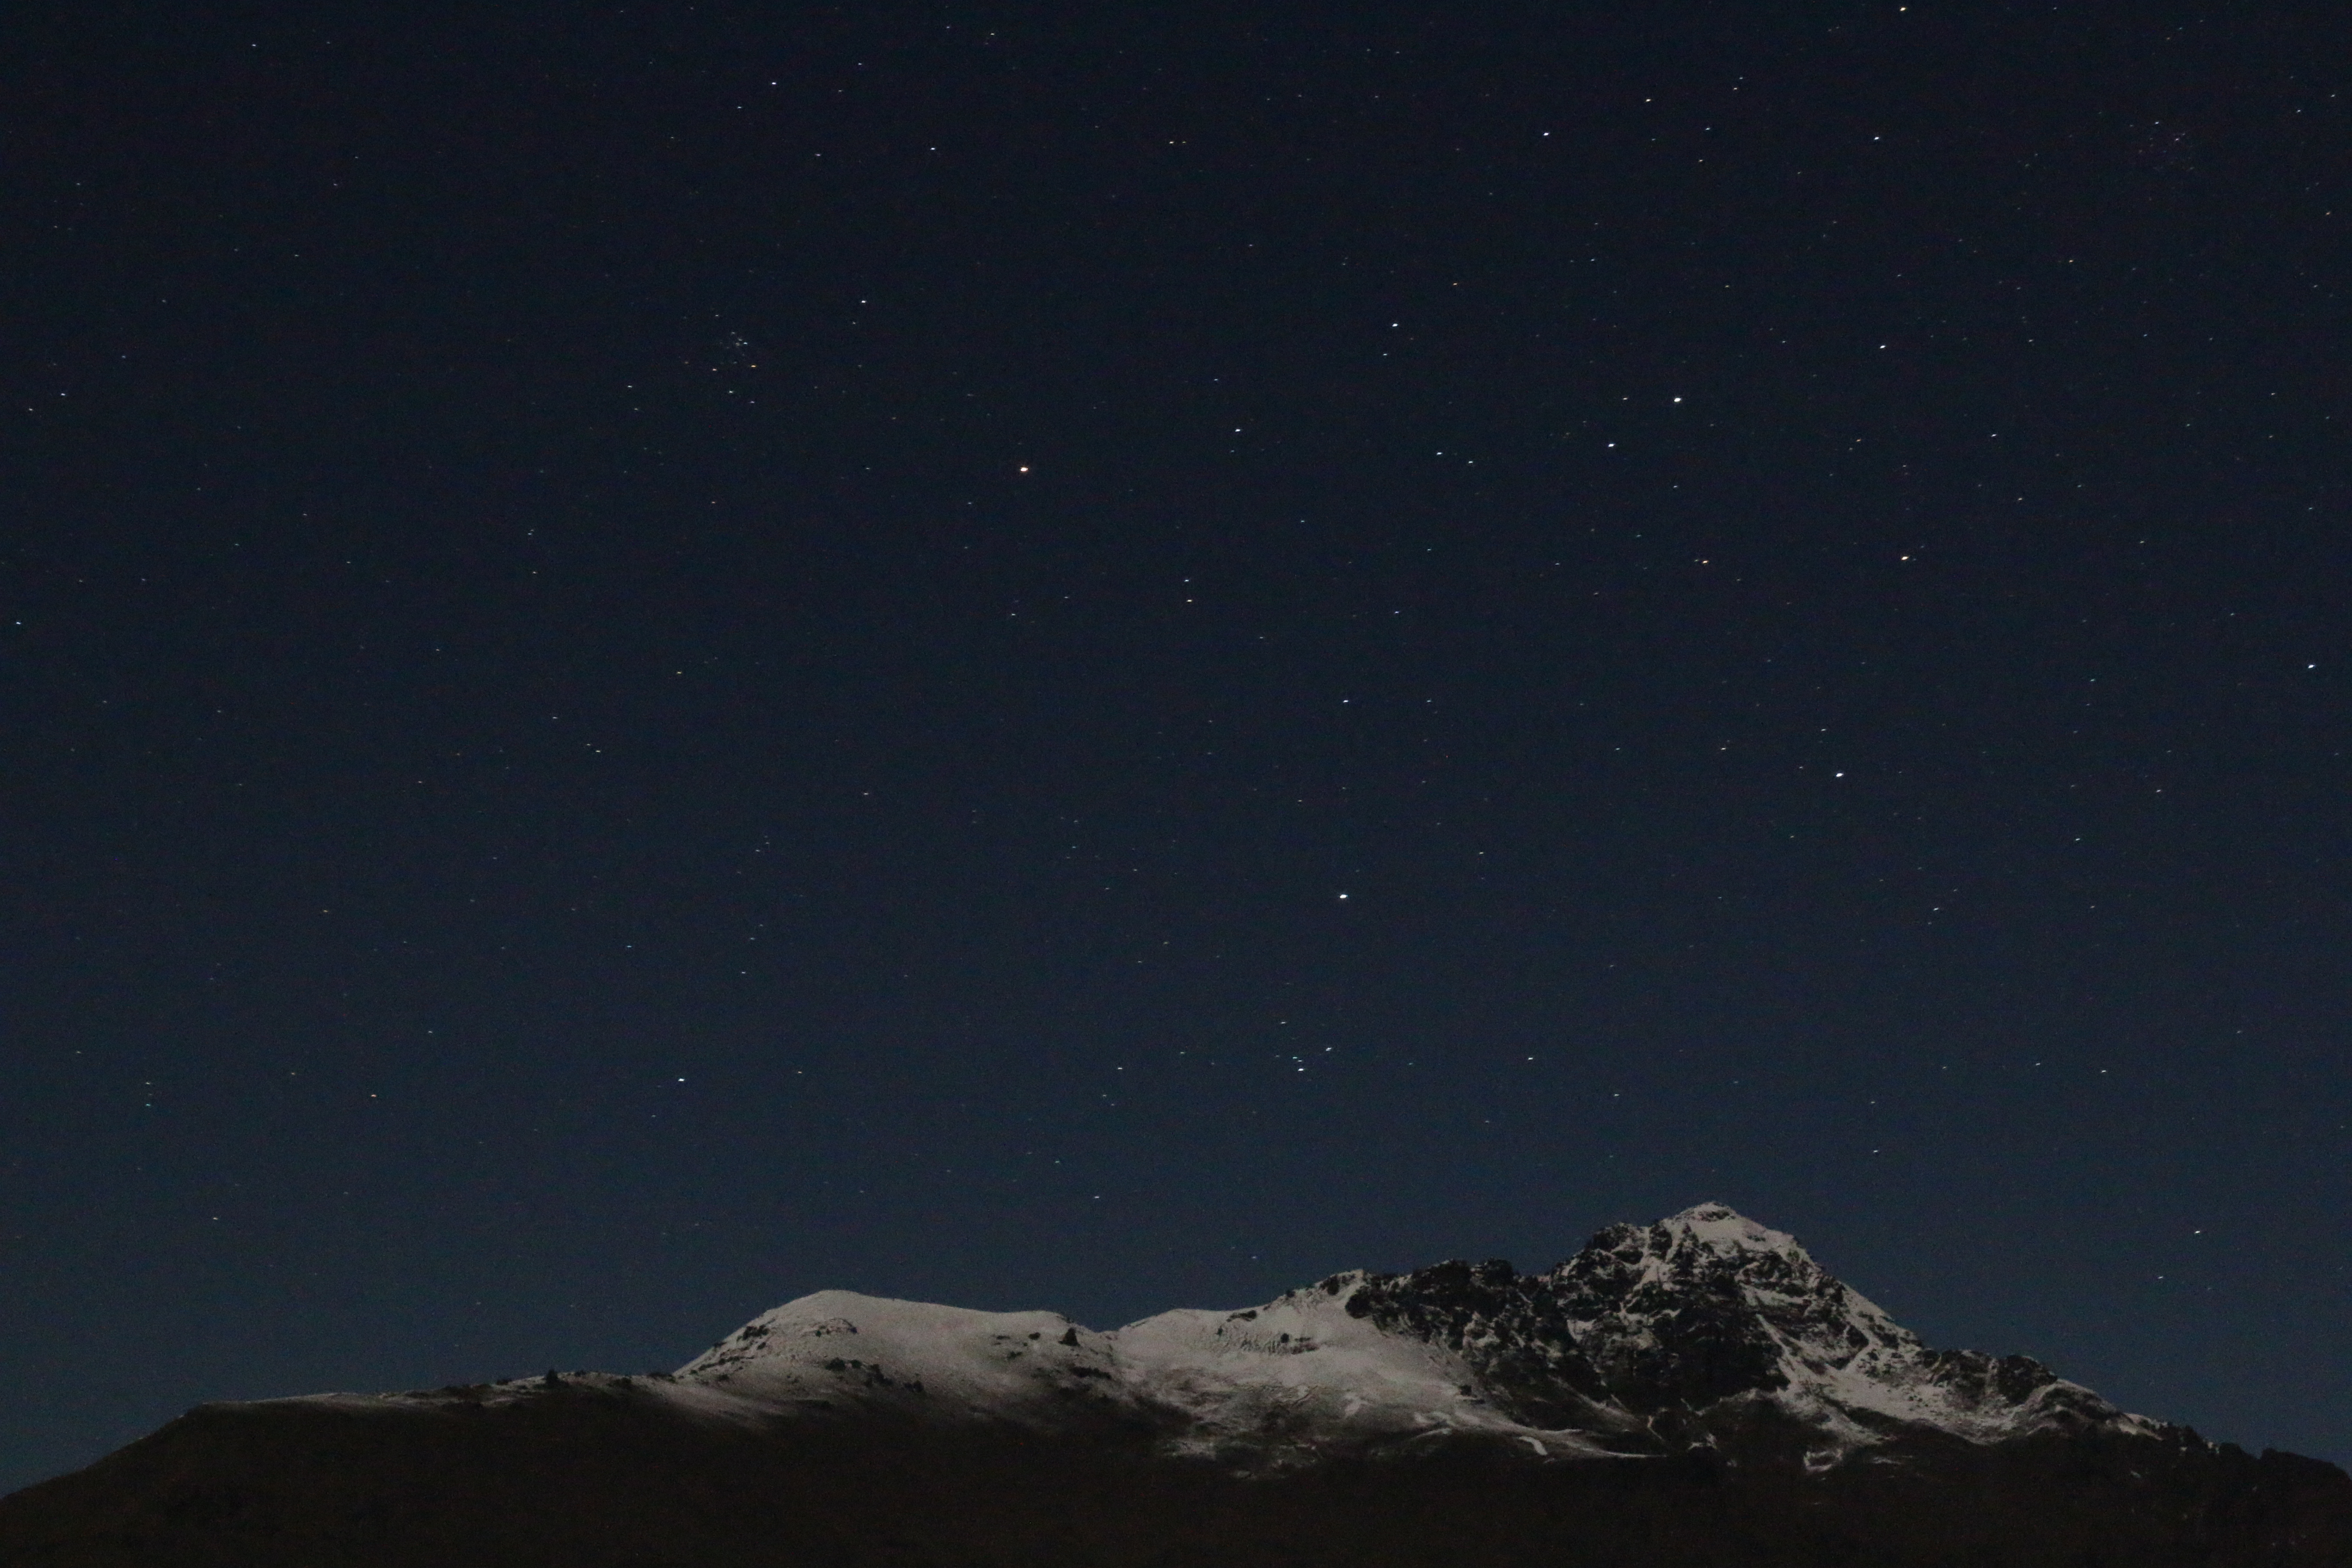
\includegraphics[height=0.5\textheight]{images/clear-skies-1}<2>
                    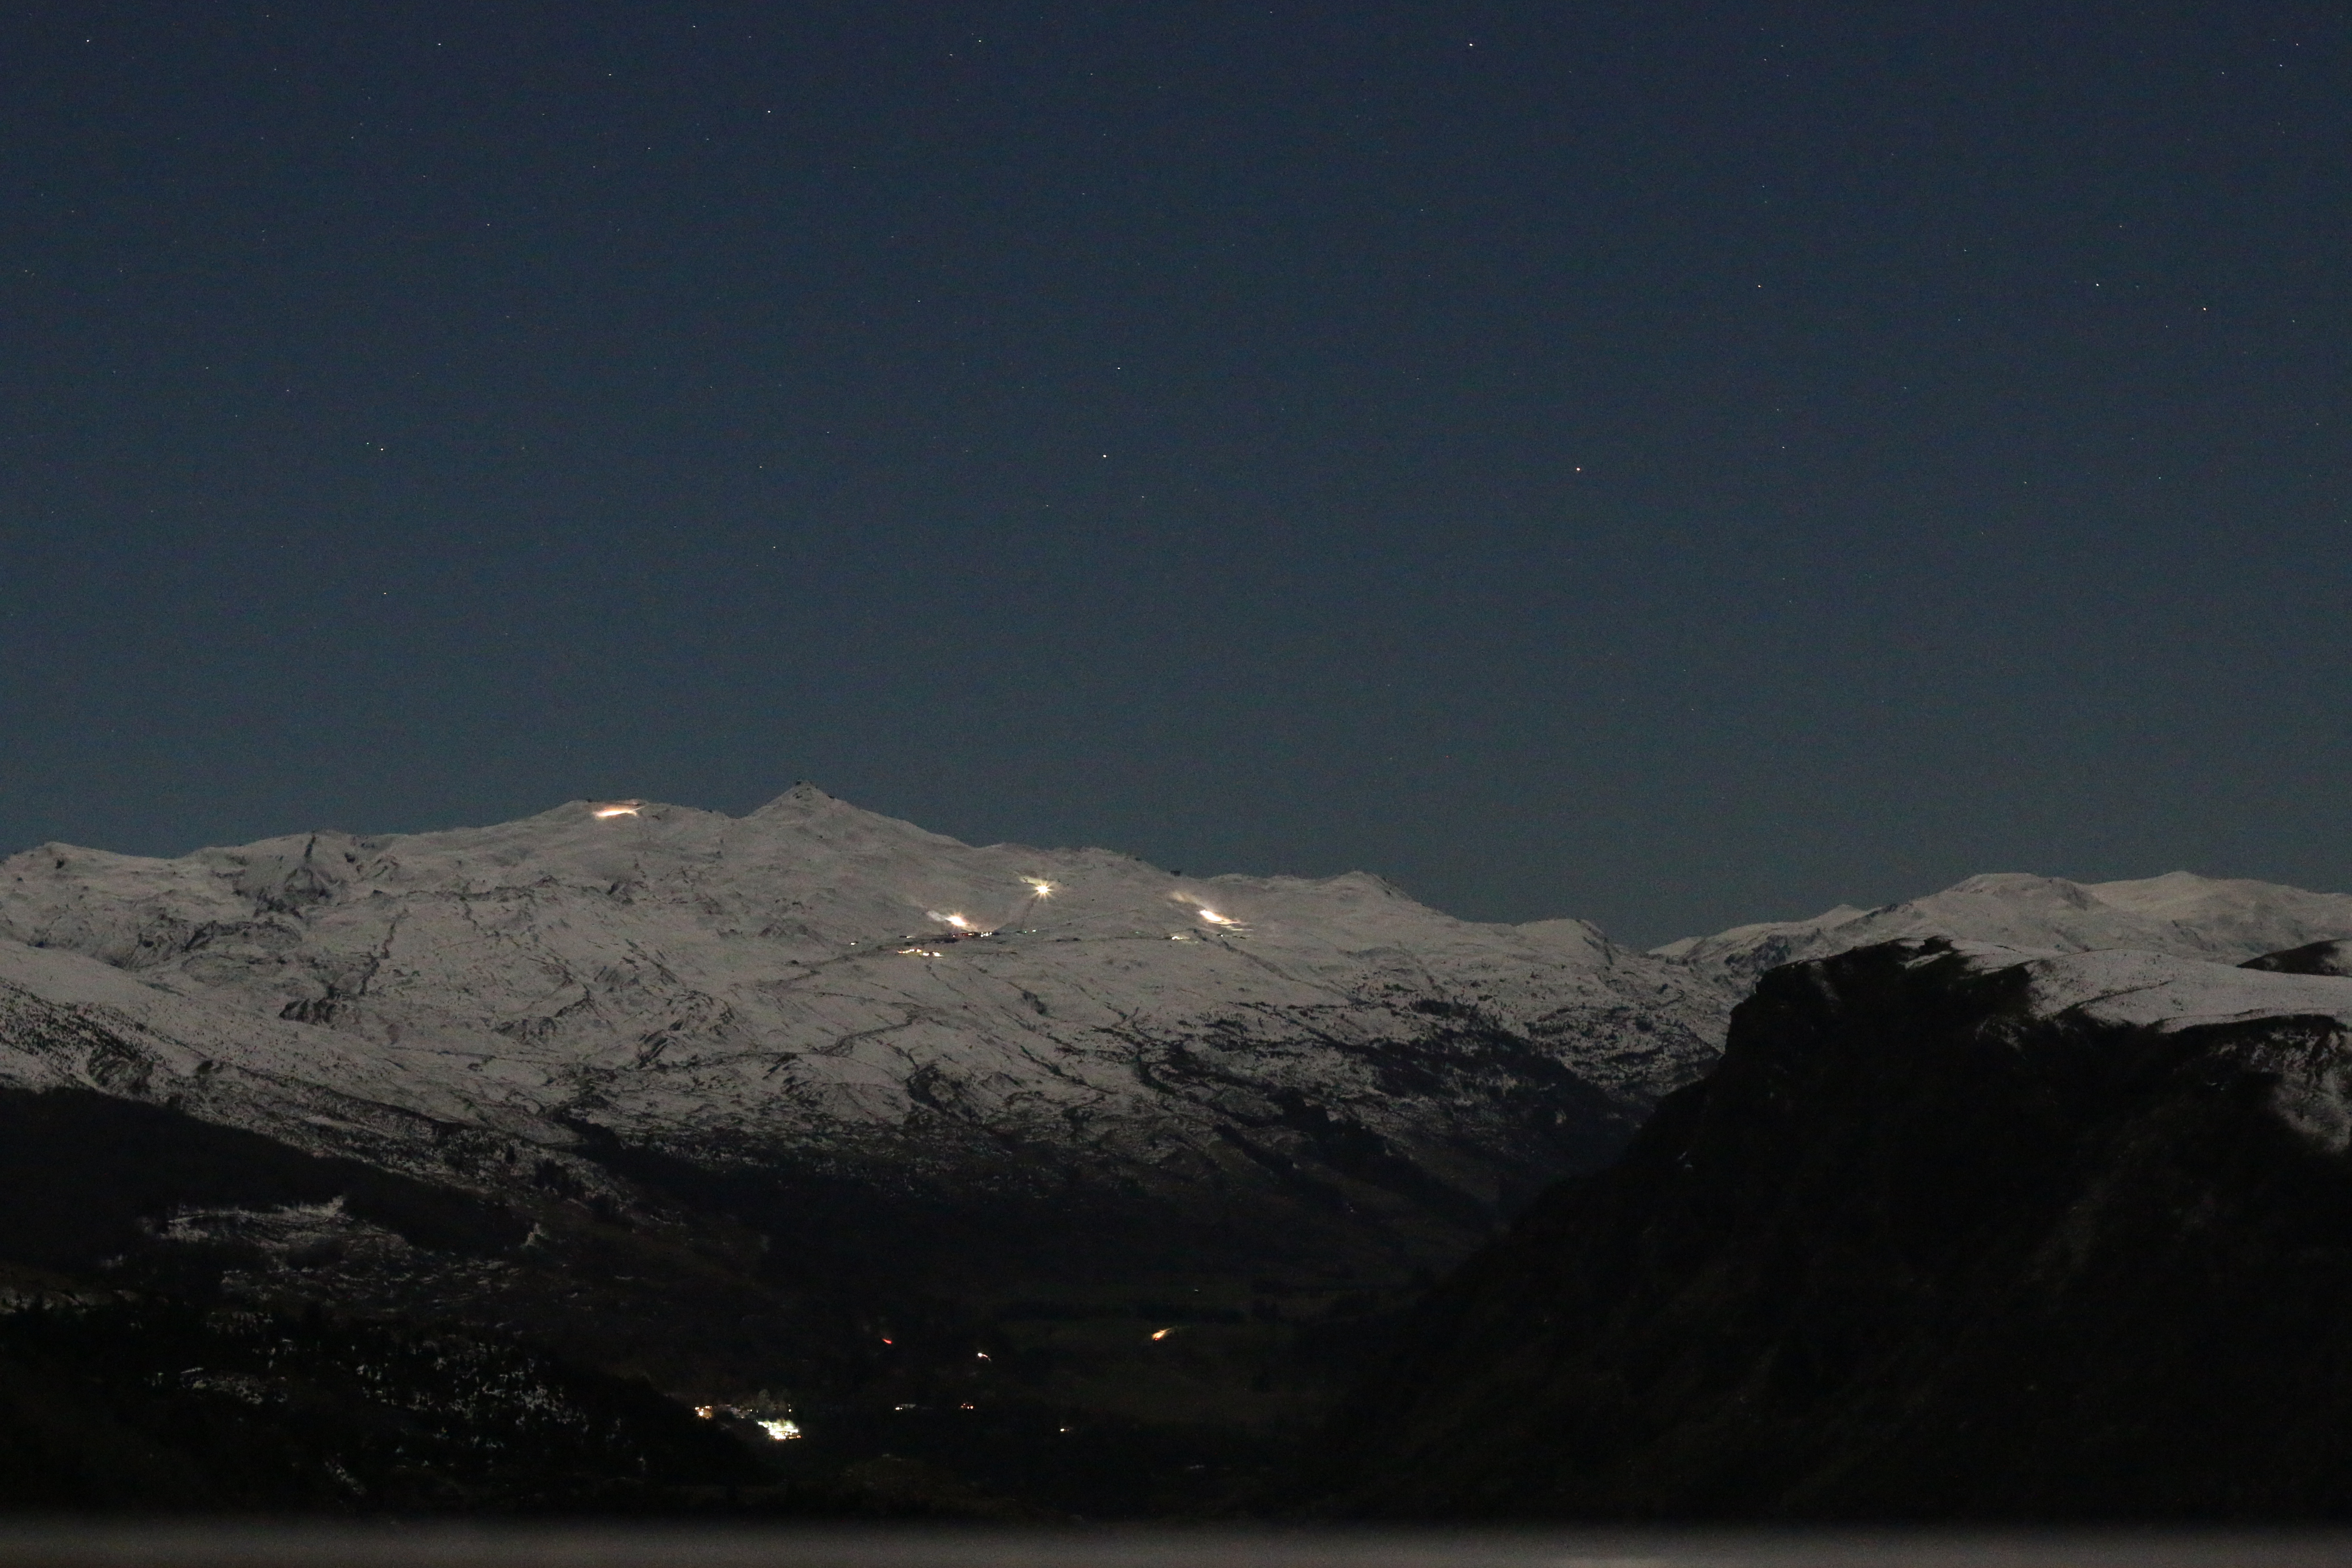
\includegraphics[height=0.5\textheight]{images/night-skies.JPG}<3>
                    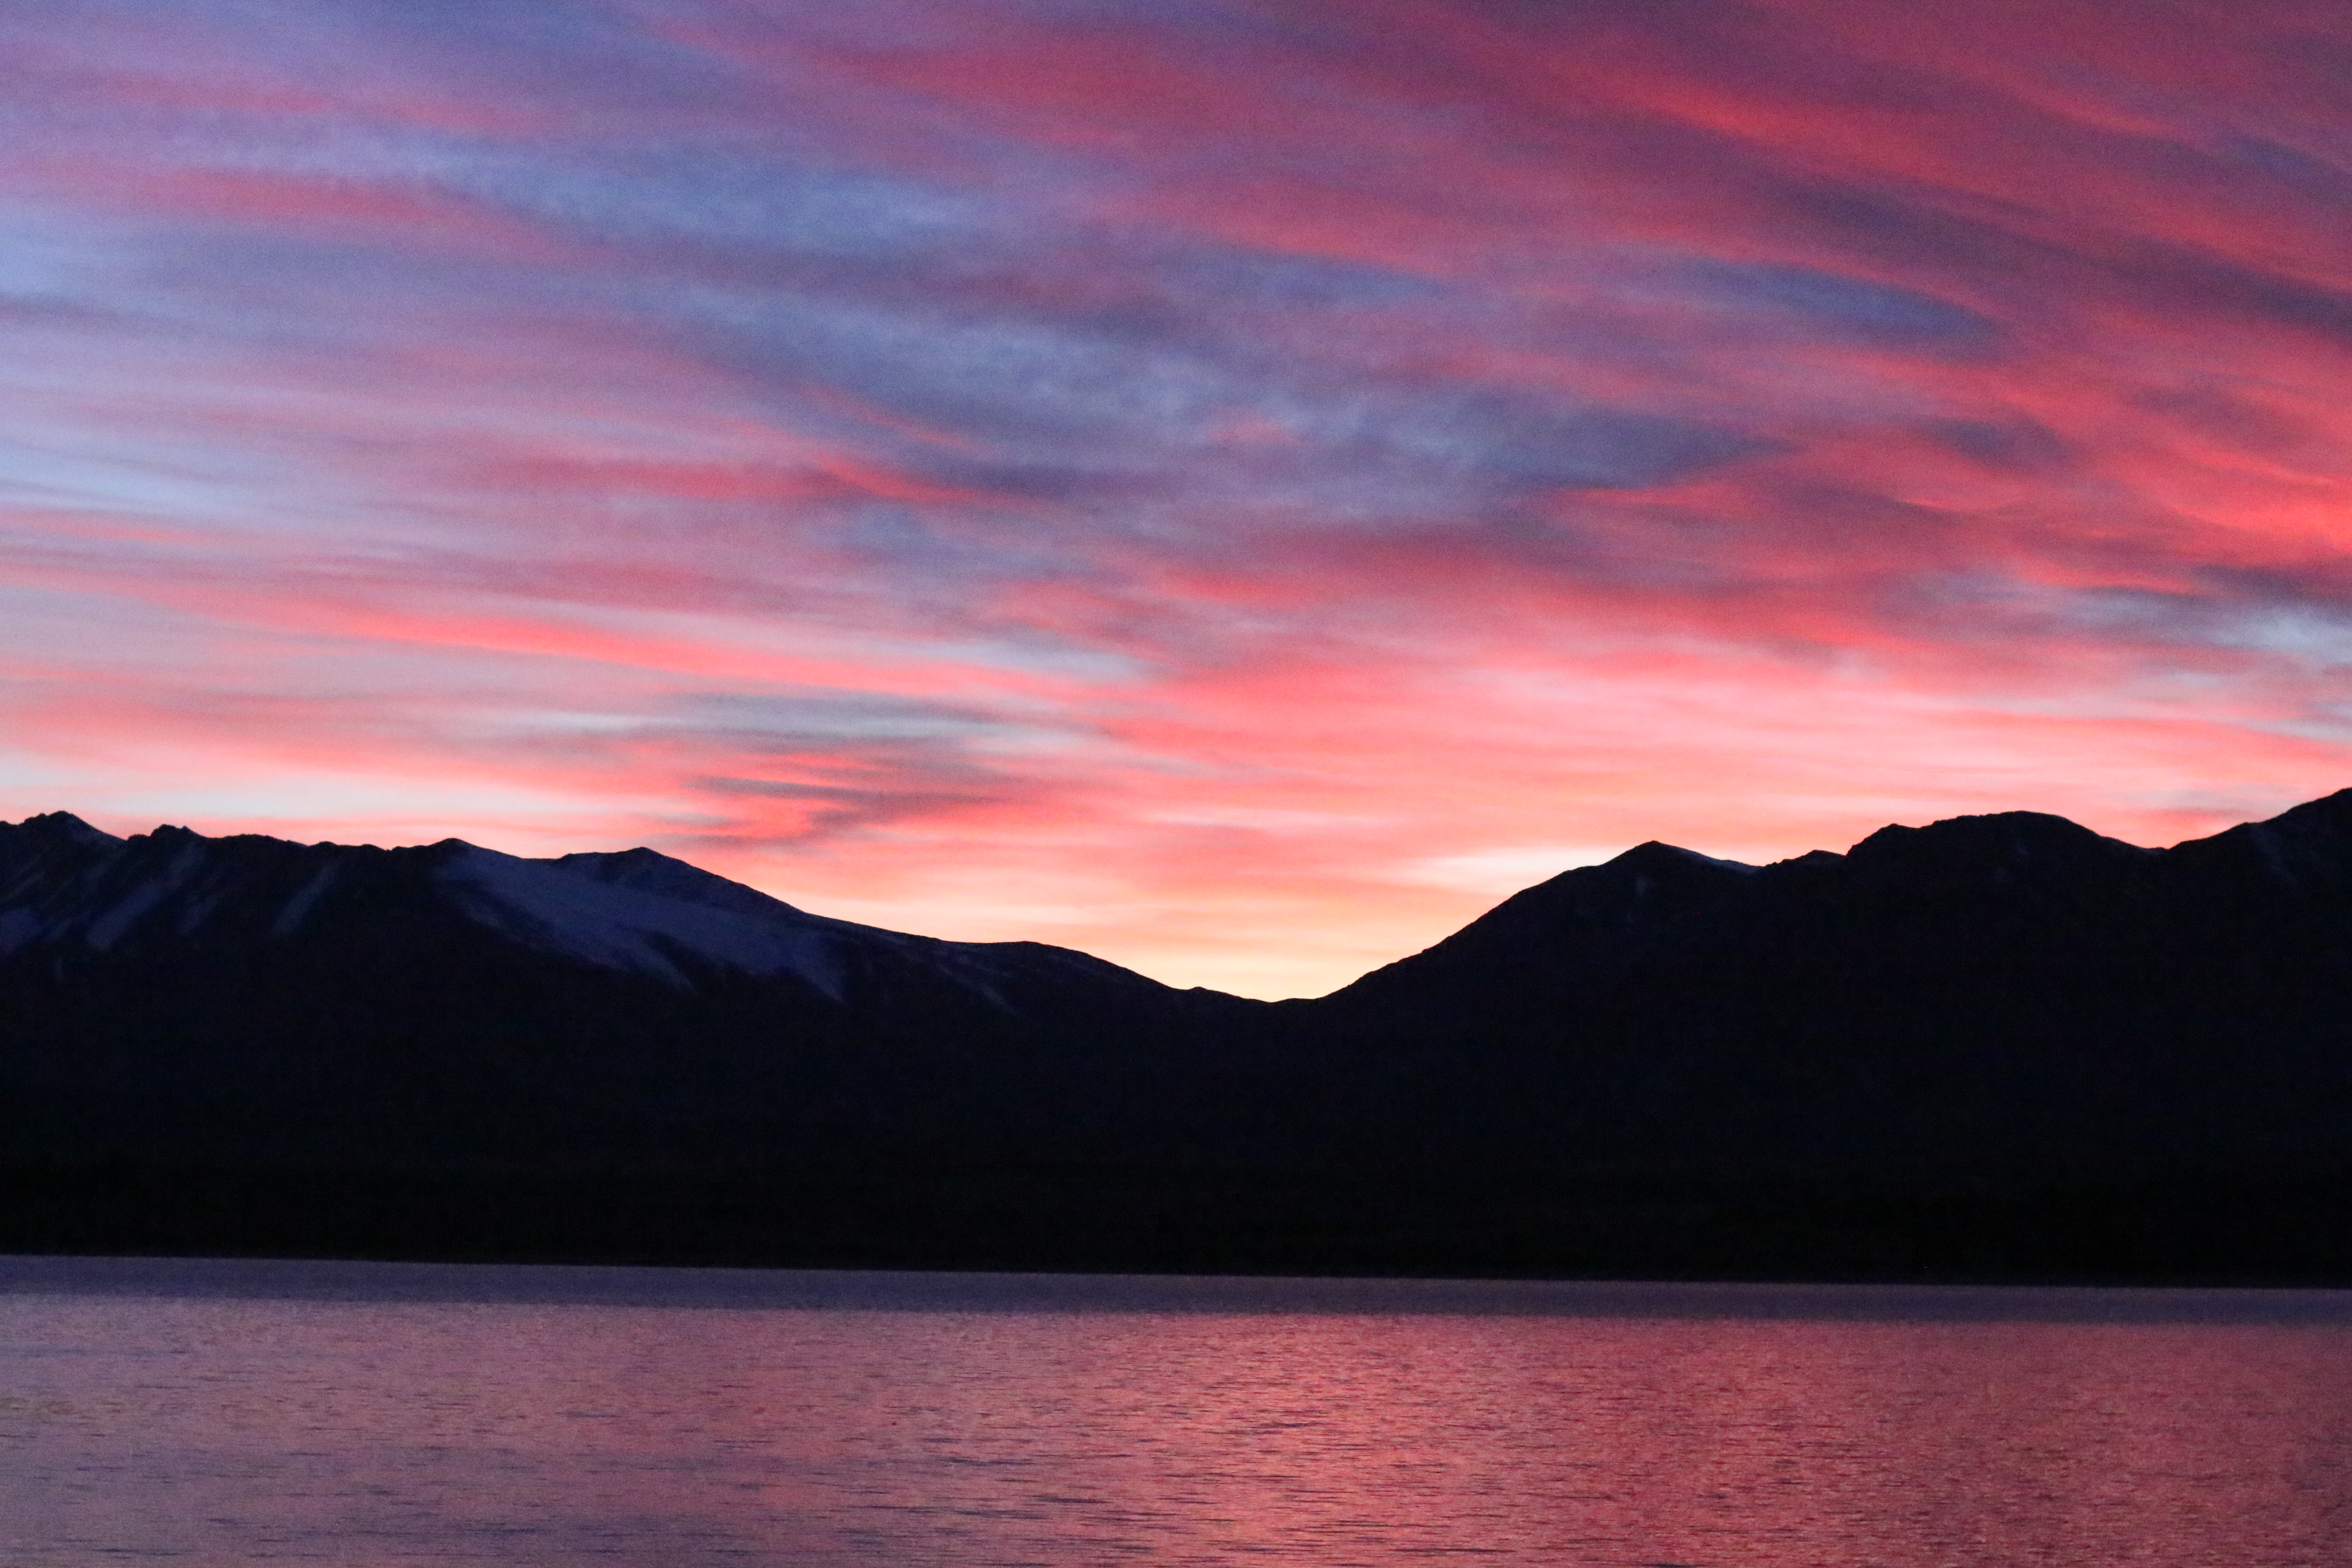
\includegraphics[height=0.5\textheight]{images/sunset.JPG}<4>
                \end{center}
            
                %\column{0.6\textwidth}
                \begin{itemize}
                    \item Blue pools (Light refraction on the snow-fed, icy cold water)
                    \pause
                    \item Was great for my night Photography
                    \pause
                    \item Night Skies
                    \pause
                    \item And the sunset
                \end{itemize}
            %\end{columns}
        \end{frame}

        \begin{frame}
            \frametitle{Fun activites}
            %\begin{columns}
                %\column{0.6\textwidth}
                \begin{itemize}
                    \item Lots of hiking
                    \pause
                    \item Skiing
                    \pause
                    \item Glacier heli hikes
                    \pause
                    \item Natural Springs
                    \pause
                    \item And more hiking
                \end{itemize}
            %\end{columns}
        \end{frame}

        \begin{frame}
            \frametitle{Food}
            %\column{0.5\textwidth}
            \begin{center}
                \includegraphics[height=0.5\textheight]{images/fergburger.jpg}<1>
                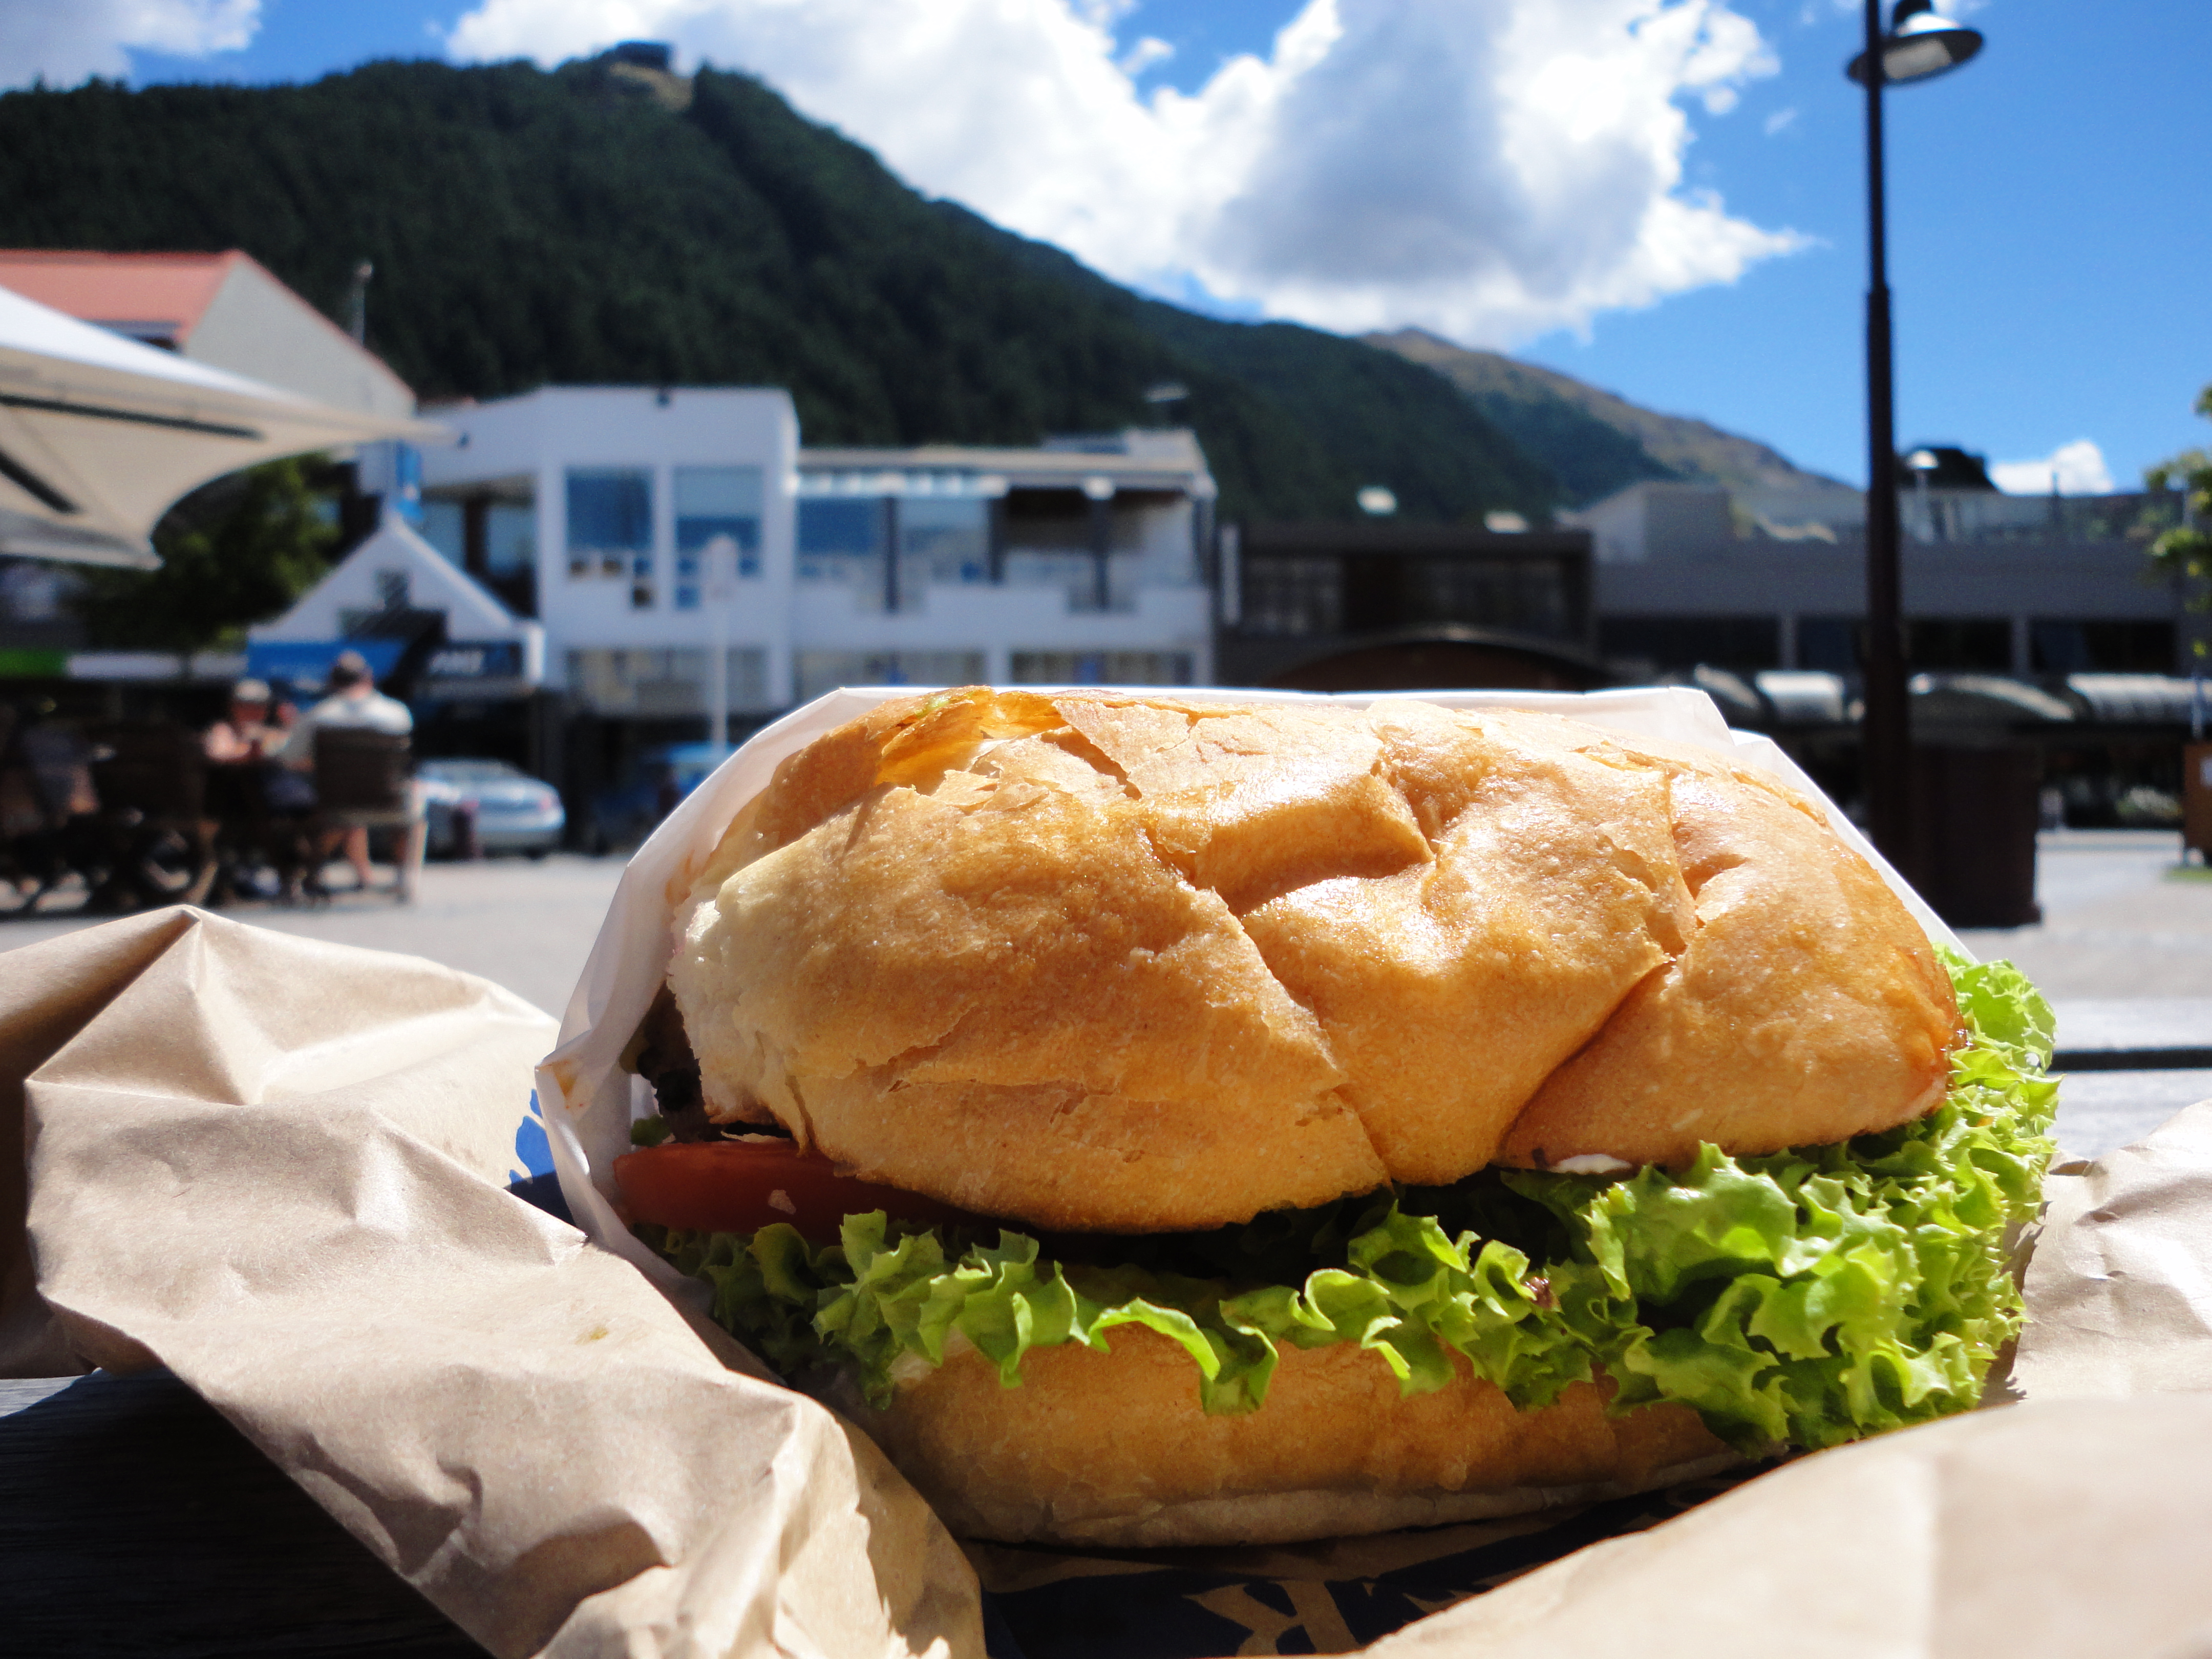
\includegraphics[height=0.5\textheight]{images/fergburger-2.jpg}<2>
                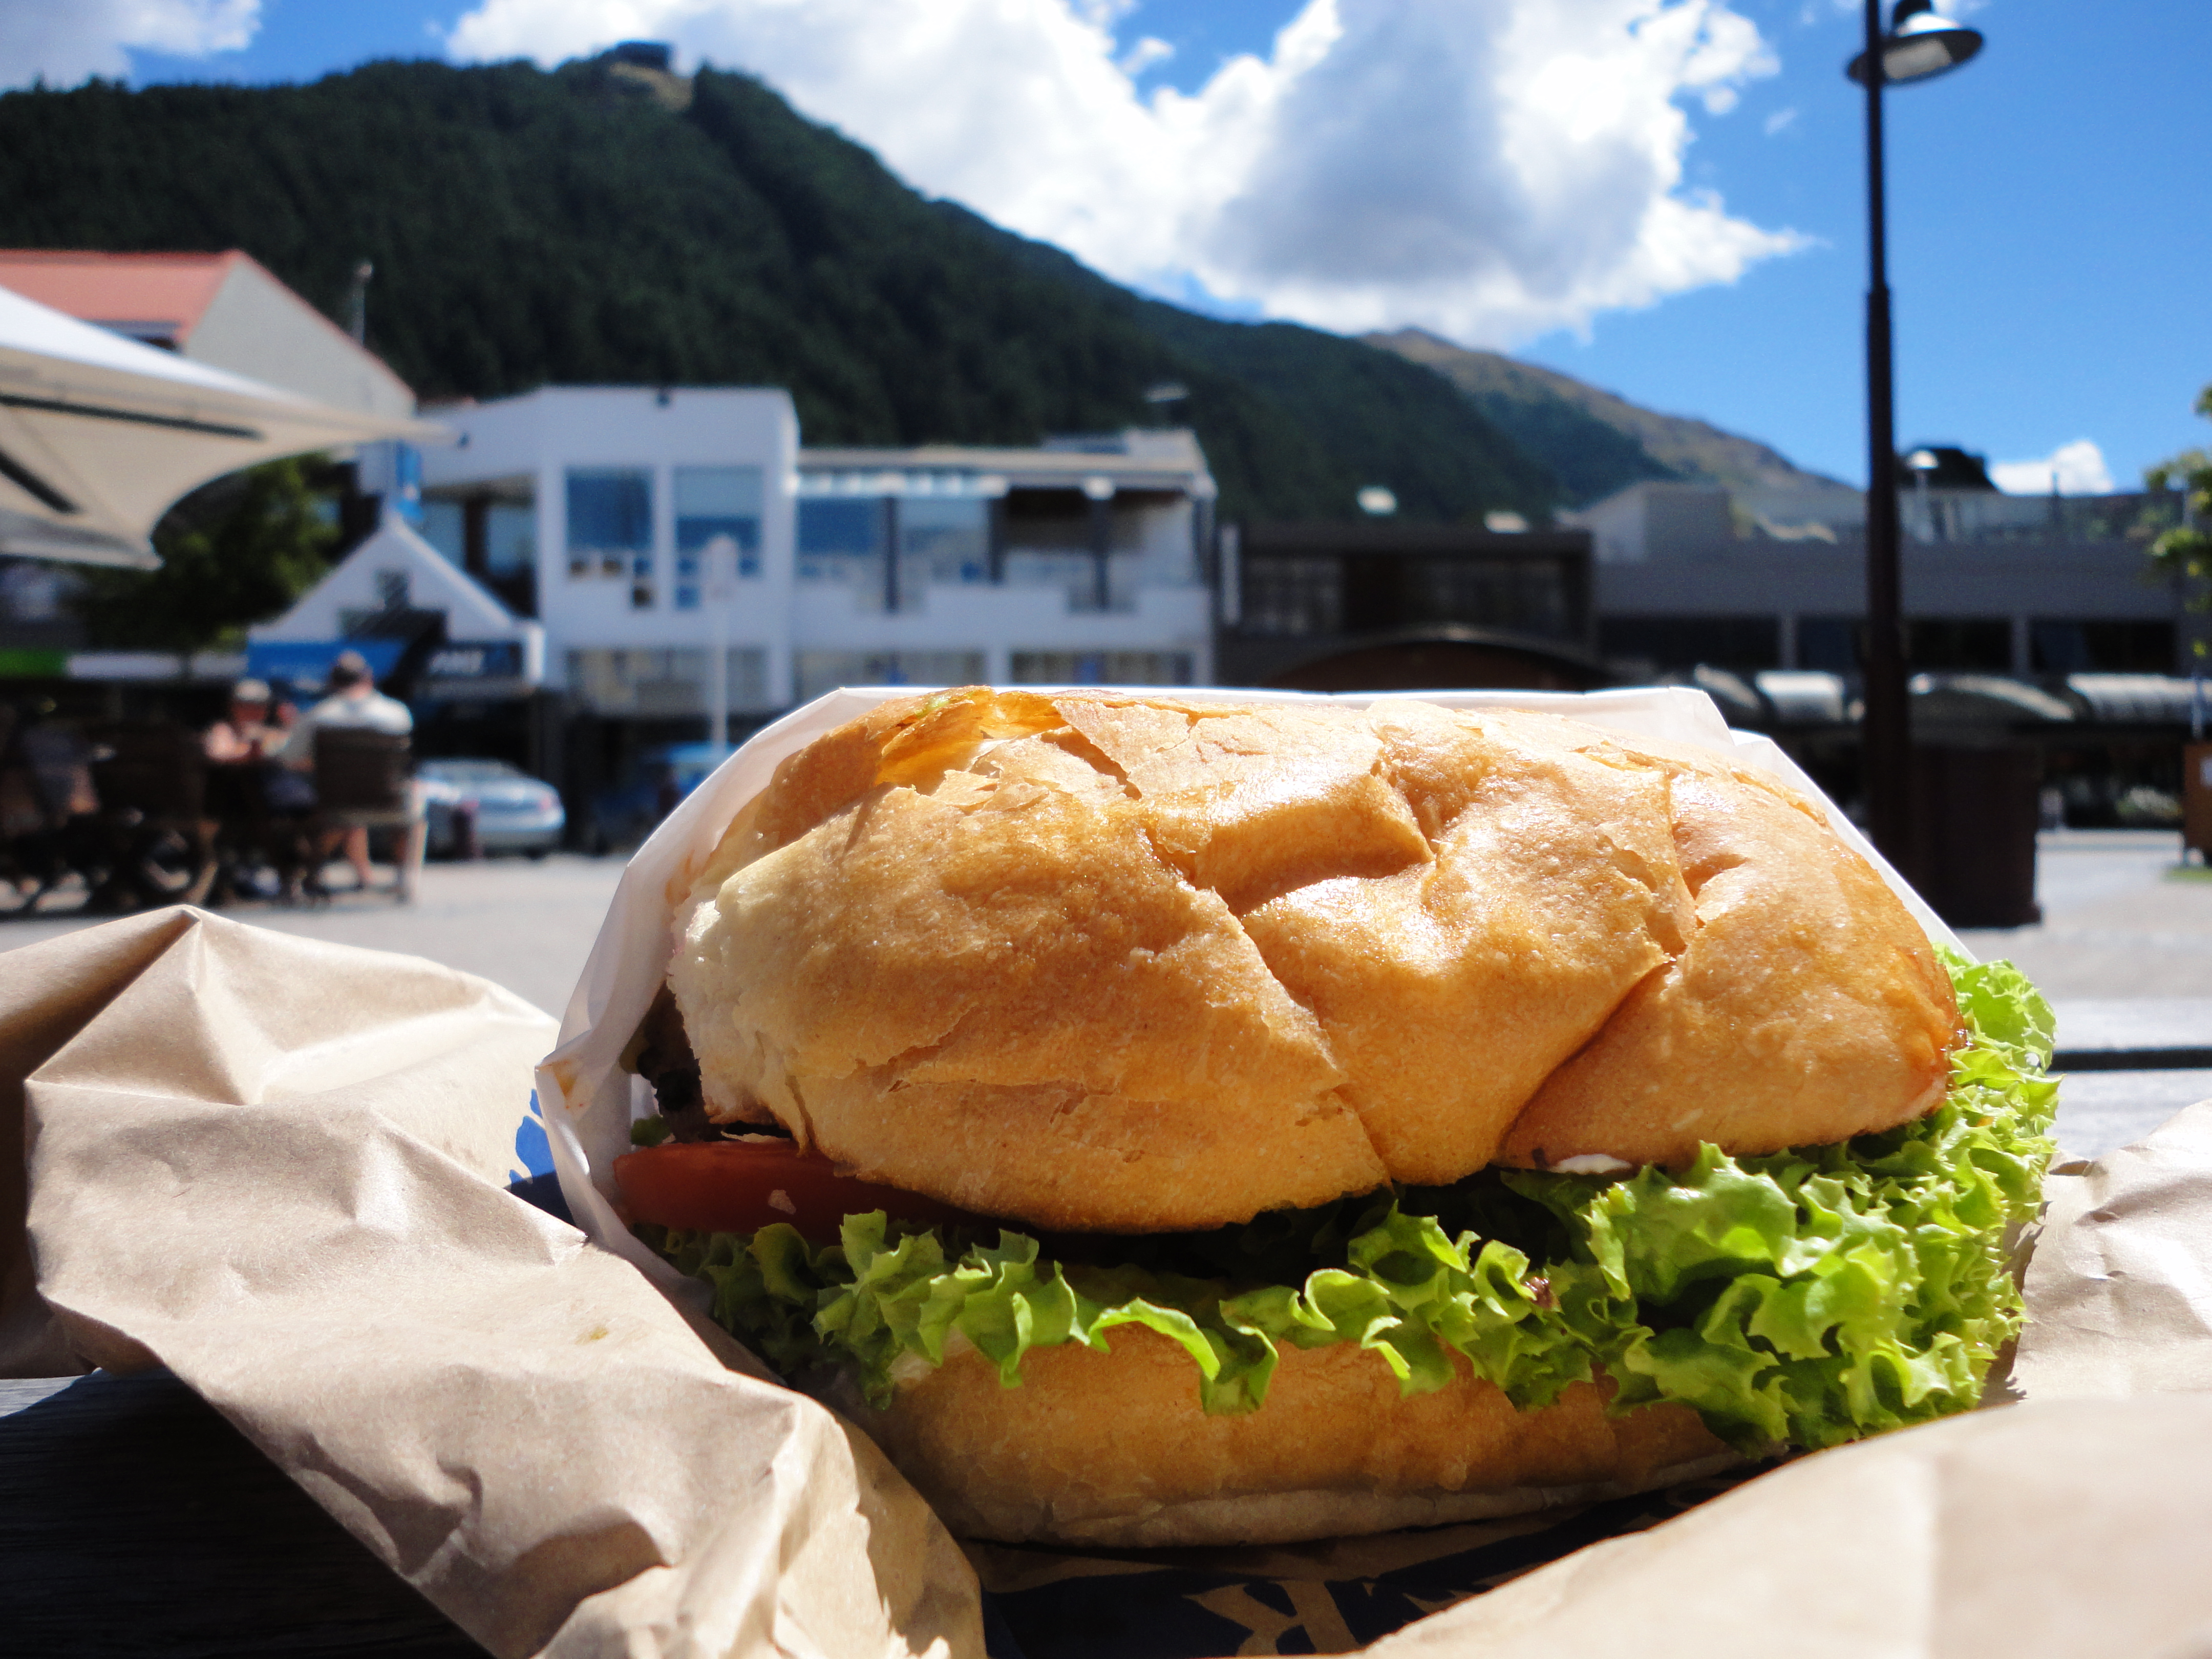
\includegraphics[height=0.5\textheight]{images/fergburger-2.jpg}<3>
                \includegraphics[height=0.5\textheight]{images/fergburger.jpg}<4>
            \end{center}

            %\begin{columns}
                %\column{0.6\textwidth}
                \begin{itemize}
                    \item Fergburger, Queenstown
                    \pause
                    \item The Best Burger in The World
                    \pause
                    \item \href{https://www.urbandictionary.com/define.php?term=Fergburger}{search Fergburger in urbandictionary}
                    \pause
                    \item after 4am in the morning and I still had to line up
                \end{itemize}
            %\end{columns}
        \end{frame}
    
    \end{document}
    